\documentclass[9pt]{beamer}
\usetheme[progressbar=head,numbering=fraction]{metropolis}
\makeatletter
\setlength{\metropolis@progressinheadfoot@linewidth}{2pt}
\definecolor{lighto}{RGB}{235,92,30}

\usepackage{empheq}
\makeatletter
\colorlet{shadecolour}{blue!30}
\newcommand\Ashaded[1]{\let\bgroup{\romannumeral-`}\@Ashaded#1&&\ENDDNE}
\def\@Ashaded#1&#2&#3\ENDDNE{%
\ifnum0=`{}\fi \setbox \z@
\hbox{$\displaystyle#1{}\m@th$\kern\fboxsep \kern\fboxrule }%
\edef\@tempa {\kern \wd\z@ &\kern -\the\wd\z@ \fboxsep
\the\fboxsep }\@tempa \colorbox{shadecolour}{$#1#2 $}%
}
\colorlet{bgcolour}{yellow!20}
\colorlet{rulecolour}{blue!30}
\newcommand\Acolorboxed[1]{\let\bgroup{\romannumeral-`}\@Acolorboxed#1&&\ENDDNE}
\def\@Acolorboxed#1&#2&#3\ENDDNE{%
  \ifnum0=`{}\fi \setbox \z@
    \hbox{$\displaystyle#1{}\m@th$\kern\fboxsep \kern\fboxrule }%
    \edef\@tempa {\kern \wd\z@ &\kern -\the\wd\z@ \fboxsep
        \the\fboxsep\fboxrule \the\fboxrule }\@tempa \fcolorbox{rulecolour}{bgcolour}{$ #1#2 $}%
}
\makeatother

\usepackage{amsmath,amssymb,bbm}
\usepackage{colortbl}
\usepackage{color}
\usepackage[latin1]{inputenc}
\usepackage[T1]{fontenc}
\usepackage{psfrag}
\usepackage[english]{babel}
\usepackage{graphicx}
\usepackage{multicol}
\usepackage{multirow}
\usepackage{tabularx}
\renewcommand{\d}{\delta}
\renewcommand{\a}{\alpha}
\newcommand{\e}{\varepsilon}
\newcommand{\F}{{\cal F}}
\newcommand{\s}{\sigma}
\newcommand{\Fd}{{\bf{F}}}
\def\P{\mathbbm P}
\newcommand{\R}{\mathbbm{R}}
\newcommand{\N}{\mathbbm{N}}
\newcommand{\un}{{\mathbbm{1}}}
\newcommand{\eqdef}{\stackrel{\Delta}{=}}
\newcommand{\E}{\mathbb E}
\newtheorem{defn}{Definition}
\newtheorem{thm}{Theorem}
\newtheorem{lem}{Lemma}
\newtheorem{cor}{Corollary}
\newtheorem{pro}{Proposition}
\newtheorem{prop}{Properties}

\definecolor{darkgreen}{rgb}{0.2,0.7,0.2}
\definecolor{nicegreen}{rgb}{0,0.667,0}
\definecolor{lightgreen}{rgb}{.667,1,.5}
\definecolor{lightblue}{rgb}{0,0.667,1}
\definecolor{orange}{rgb}{1,.333,0}
\definecolor{maroon}{rgb}{0.75,.25,0}
\definecolor{pink}{rgb}{1,0,1}
\definecolor{darkgray}{gray}{.3}
\newcommand{\white}[1]{\textcolor{white}{#1}}
\newcommand{\red}[1]{\textcolor{red}{#1}}
\newcommand{\blue}[1]{\textcolor{blue}{#1}}
\newcommand{\green}[1]{\textcolor{green}{#1}}
\newcommand{\black}[1]{\textcolor{black}{#1}}
\newcommand{\nicegreen}[1]{\textcolor{nicegreen}{#1}}
\newcommand{\lightgreen}[1]{\textcolor{lightgreen}{#1}}
\newcommand{\lightblue}[1]{\textcolor{lightblue}{#1}}
\newcommand{\lightgray}[1]{\textcolor{lightgray}{#1}}
\newcommand{\pink}[1]{\textcolor{pink}{#1}}
\newcommand{\orange}[1]{\textcolor{orange}{#1}}
\newcommand{\maroon}[1]{\textcolor{maroon}{#1}}
\newcommand{\darkgray}[1]{\textcolor{darkgray}{#1}}
\newcommand{\yellow}[1]{\textcolor{yellow}{#1}}

\newcommand{\rank}[1]{\operatorname{rank}\p{#1}}
\newcommand{\nn}{\mathcal{N}}
\newcommand{\Norm}[1]{\left\lVert#1\right\rVert}
\newcommand{\argmin}{\operatorname{argmin}}
\newcommand{\law}{\mathcal{L}}
\newcommand{\EE}[2][]{\mathbb{E}_{#1}\left[#2\right]}
\newcommand{\simiid}{\,{\buildrel \text{iid} \over \sim\,}}
\newcommand{\p}[1]{\left(#1\right)}
\newcommand{\cX}{{\mathcal X}}%
\newcommand{\cY}{{\mathcal Y}}
\def\rset{\ensuremath{\mathbb{R}}}
\newcommand{\eqsp}{\;}

\newcommand{\calF}{\mathcal{F}}


\AtBeginSection[]
{
  \begin{frame}
      \frametitle{Outline}
      \tableofcontents[currentsection]
 \end{frame}
}

\AtBeginSubsection[]
{
   \begin{frame}
       \frametitle{Outline}
       \tableofcontents[currentsection,currentsubsection]
   \end{frame}
}

\title[Introduction to machine learning]{{\em MAP 534} \\
Introduction to machine learning\\}
\author{}
\date{}

\begin{document}

\author[S. Le Corff]{\textcolor{violet}{Dimension reduction}\\ {\em {\small \textcolor{violet}{Principal component analysis (PCA) \& Kernel PCA}}}}

%\begin{frame}[t]
%
%\medskip
%
%
%\begin{center}
%\LARGE
%
%%\textcolor{lighto}{MSc Data Science for Business}
%
%%\rule{4cm}{2pt}
%
%\vspace{2.2cm}
%
%\textcolor{violet}{{\bf Introduction to Machine Learning}}
%
%\medskip
%
%\textcolor{violet}{MAP 534}
%
%\end{center}
%
%\medskip
%
%\medskip
%
%\begin{center}
%  {\em \textcolor{lighto}{Sylvain Le Corff}}
%
%  \medskip
%
% %\includegraphics[width=3cm]{X.jpg}
%\end{center}
%\end{frame}

\begin{frame}
  \maketitle 
\end{frame}

\section{Machine learning in a few words}

\begin{frame}{Machine Learning in a few words}
%Machine learning problems can be decomposed into two different classes.

\textcolor{lighto}{{\bf Classification}}


$\rightharpoondown$  Learn whether \textcolor{violet}{an individual from $\mathbb{R}^d$ belongs to some class}. 

$\rightharpoondown$  Focus usually set on learning with a \textcolor{violet}{known number $M$ of classes}:  an individual is associated with a label in $\{1,\ldots,M\}$. 

$\rightharpoondown$  The statistical model is then given by $(X,Y)\in\mathbb{R}^p\times \{1,\ldots,M\}$ and the objective is to \textcolor{violet}{define a function $f: \mathbb{R}^p \to \{1,\ldots,M\}$, called classifier, such that $f(X)$ is the best prediction of $Y$ in a given context}.

\vspace{.5cm}

\textcolor{lighto}{{\bf Regression}}



$\rightharpoondown$ \textcolor{violet}{The observation associated with $X$} is assumed to be given by
$$
Y = f(X) + \varepsilon\,,
$$
where $\varepsilon$ is a centered noise independent of $X$. 

$\rightharpoondown$ The statistical model is then given by $(X,Y)\in\mathbb{R}^p\times \mathbb{R}^m$ and \textcolor{violet}{the objective is to define the  best estimator of $f$ in a given context}. %An element of $\mathbb{R}^p$ contains all the features the label prediction or the regression estimate has to be based on.
\end{frame}

\begin{frame}{Machine Learning in a few words - clustering}
\begin{center}
%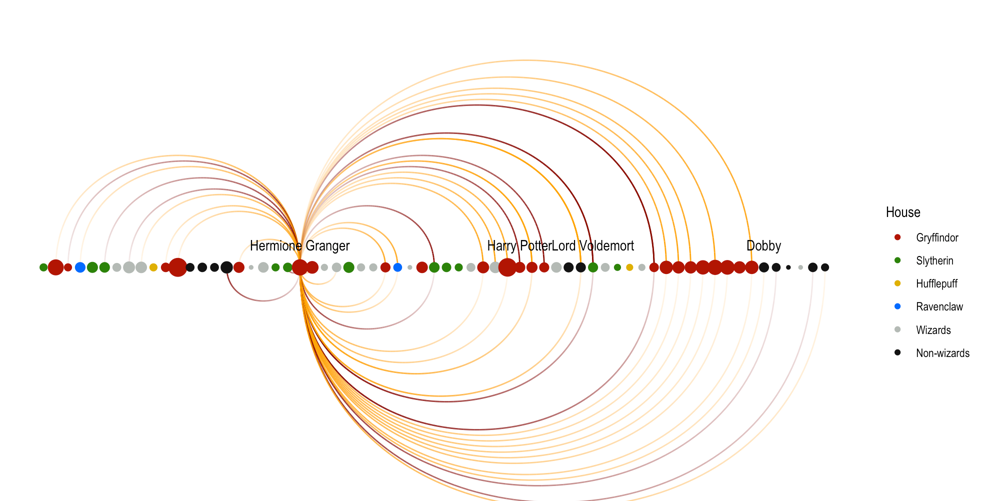
\includegraphics[scale=.2]{hp.png}
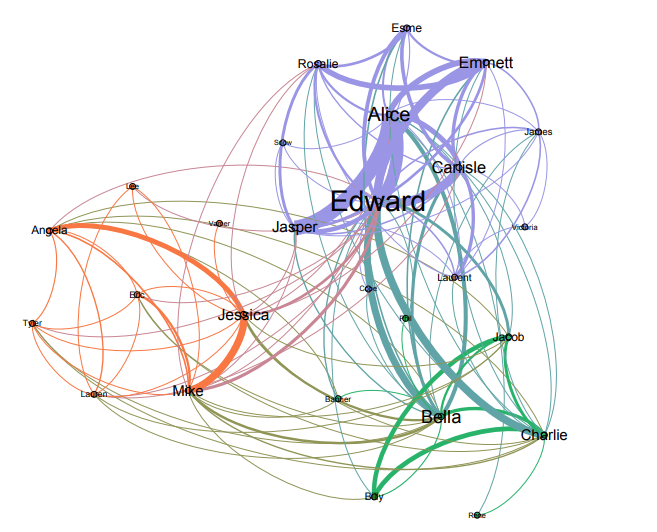
\includegraphics[scale=.2]{twlght.png}
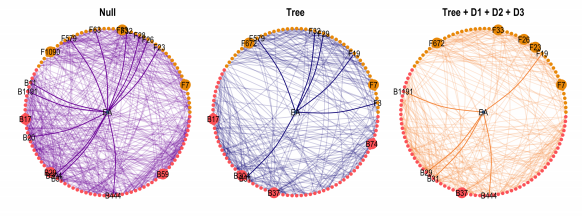
\includegraphics[scale=.45]{network.png}
\end{center}

\vspace{-.4cm}

$\rightharpoondown$  \alert{Task}: group characters/news in texts/journals, infer an ecological network\footnote{{\tiny Tree-based Reconstruction of Ecological Network from Abundance Data, {\bf Momal, R. et al.}, {\em ArXiv:1905.02452}}}.

%\vspace{-.1cm}

$\rightharpoondown$  \alert{Performance}: quality of the clusters.

%\vspace{-.1cm}

$\rightharpoondown$  \alert{Experience}:  number of occurrences of two key names both within a specified distance in the text /  abundance of all species  in all sites.

\end{frame}

\begin{frame}{Machine Learning in a few words - object recognition}

%\textcolor{violet}{{\bf A detection/recognition algorithm.}}

\begin{center}
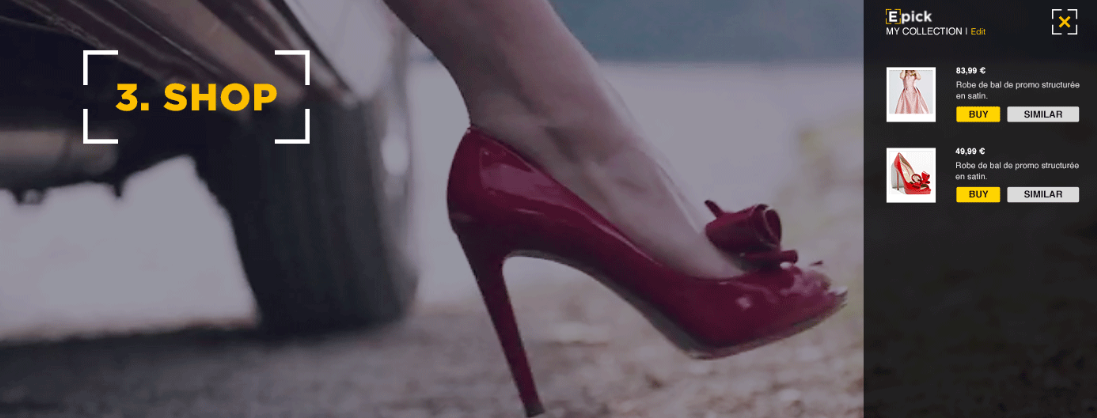
\includegraphics[width=.75\textwidth]{watiz_ex.PNG}
\end{center}

\vspace{.2cm}

$\rightharpoondown$   \alert{Task}: say if an object is present or not in the image.

$\rightharpoondown$  \alert{Performance}: number of errors.

$\rightharpoondown$  \alert{Experience}: set of previously seen labeled images.

\end{frame}

\begin{frame}{Machine Learning in a few words - prediction of time series}
\begin{center}
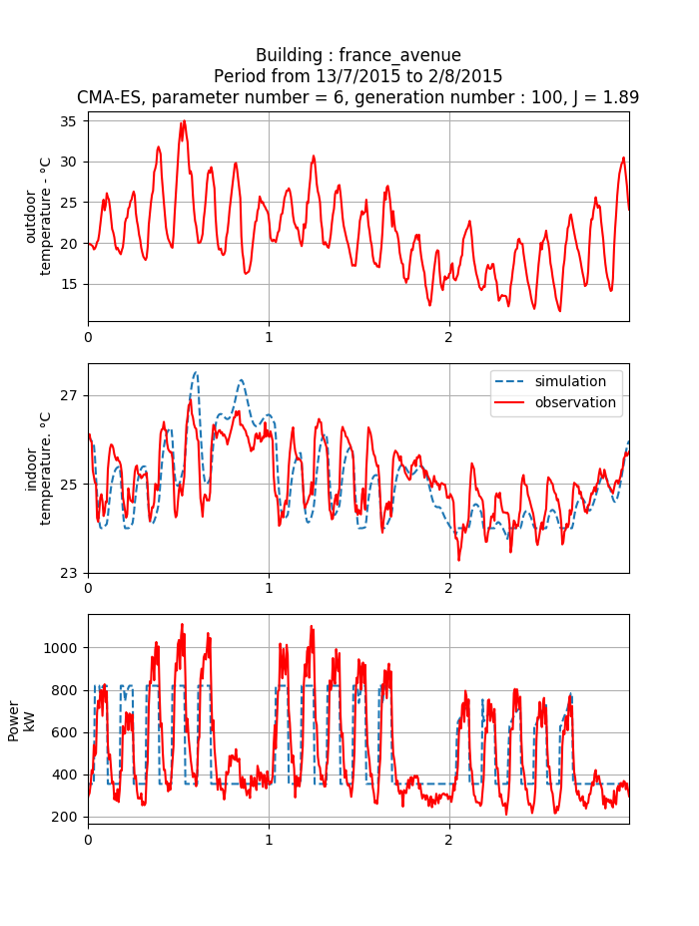
\includegraphics[scale = .3]{caliboze.png}
\raisebox{1.2cm}{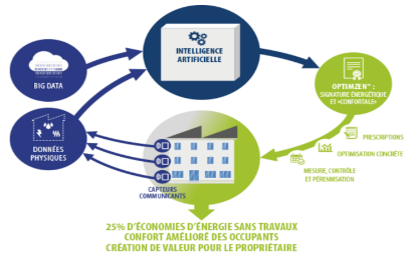
\includegraphics[scale = .35]{oze.png}}
\end{center}

$\rightharpoondown$ \alert{Task}: predict future consumptions, gas emissions and temperatures.

$\rightharpoondown$ \alert{Performance}: comfort/ecological scores.

$\rightharpoondown$ \alert{Experience}: millions of observations obtained from hundreds of sensors.

\end{frame}


\begin{frame}\frametitle{Machine Learning in a few words}
\begin{center}
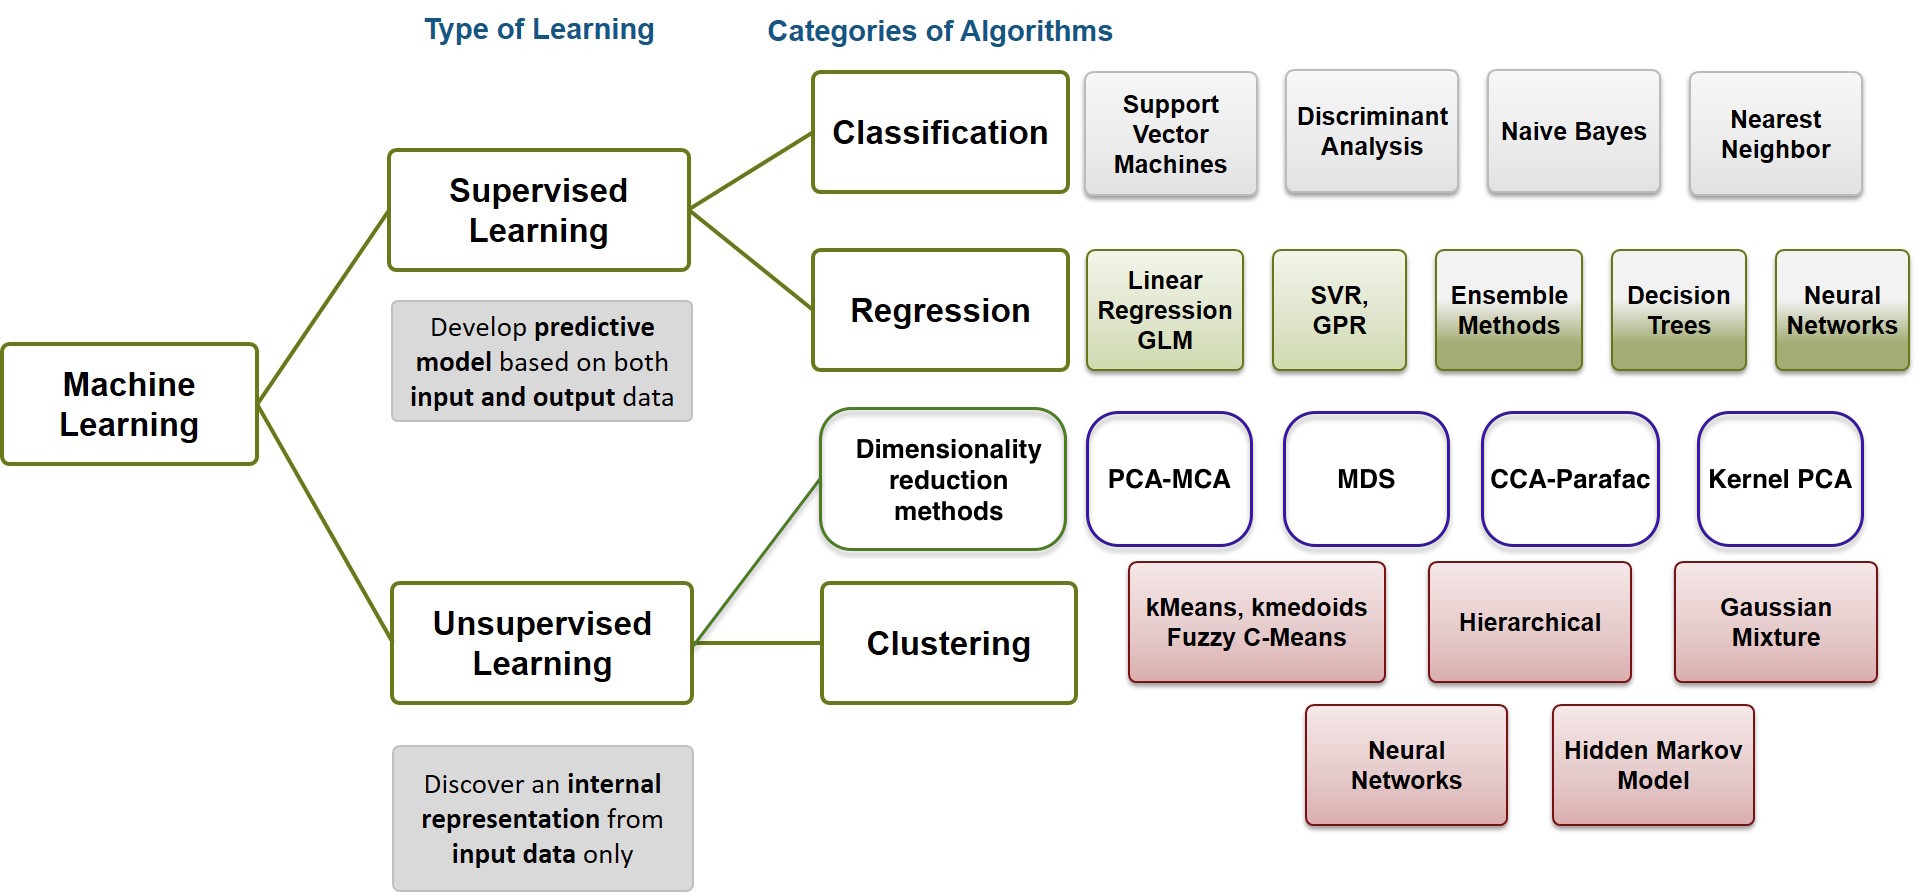
\includegraphics[width=\textwidth]{./Learning+Types.jpg}
\end{center}
\end{frame}

\begin{frame}{MAP 534 - Objectives}

$\rightharpoondown$ Master the \alert{statistical learning} framework and its challenges.

$\rightharpoondown$ Know the inner mechanism of some classical \alert{machine learning methods}.\\
{\em {\small Principal component analysis, Logistic regression, Support Vector Machines, Neural networks, gradient descent}}.

$\rightharpoondown$ Know how to implement (\alert{R and Python}) the most classical \alert{learning} algorithms.

$\rightharpoondown$ Understand some \alert{optimization} tools used in ML as well as some \alert{theoretical aspects} of ML.

\vspace{.5cm}

\textcolor{violet}{{\bf Evaluation}}

$\rightharpoondown$ A practical lab on optimization (5 pt).

$\rightharpoondown$ A final exam (15 pt).

\end{frame}

\begin{frame}{MAP 534 - Team}

\textcolor{violet}{{\bf Lectures}}: \textcolor{lighto}{Sylvain Le Corff}
\begin{center}
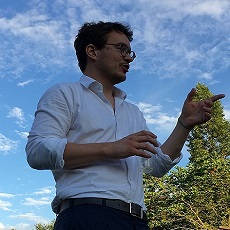
\includegraphics[scale=.4]{portrait}
\end{center}

\textcolor{violet}{{\bf Practical sessions}}: \textcolor{lighto}{Thomas Kerdreux, Sylvain Le Corff}
\begin{center}
%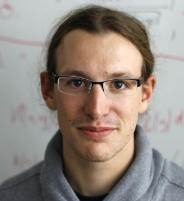
\includegraphics[scale = .5]{dieuleveut}

\includegraphics[scale = .8]{kerdreux}
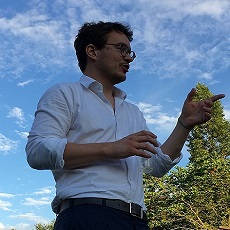
\includegraphics[scale=.4]{portrait}
\end{center}



\end{frame}

%
%%%%%%%%%%%%%%%%%%%%%%%%%%%%%
%\frame
%%%%%%%%%%%%%%%%%%%%%%%%%%%%%
%{ \frametitle{Outline}
%\vfill
%  \textbf{Supervised learning }
%  \begin{itemize}
%    \item We have training data $D_n = [(x_1, y_1), \ldots, (x_n, y_n)]$
%     \item Construct a predictor $\hat f : \cX \rightarrow \cY$ using $D_n$
%    \item Loss $\ell(y, f(x))$ measures how well $f(x)$ predicts $y$ well
%\item Aim: minimize the generalization error  \\
%  The goal is clear: predict the label $y$ based on features $x$
%\end{itemize}
%\vfill
%  \textbf{Unsupervised learning}
%  \begin{itemize}
%    \item We have training data $D_n = [x_1, \ldots, x_n]$
%    \item Loss: ????, Aim: ???? \\
%  The goal is less well defined. \\\textbf{Clustering}: construct  homogeneous groups \\
%    \textbf{Dimension reduction}: construct a map to visualize the data 
%\end{itemize}
%}
%
%%%%%%%%%%%%%%%%%%%%%%%%%%%%%
%\frame
%%%%%%%%%%%%%%%%%%%%%%%%%%%%%
%{ \frametitle{Outline}
%\vfill
%\textbf{Unsupervised learning}
%\begin{itemize}
%\item Dimensionality reduction methods (PCA)
%\item Clustering ($k$-means, Hierarchical clustering)
%\item Handling missing values/ matrix completion \\
%$\Rightarrow$ Data visualization - exploratory data analysis 
%\end{itemize}
%\vfill
%\textbf{Supervised learning}
%\begin{itemize}
%\item Theoritical framework - Bayes risk (LDA, SVM)
%\item Logistic regression
%\item Optimization
%\end{itemize}
%
%}
%
%%%%%%%%%%%%%%%%%%%%%%%%%%%%%
%\frame
%%%%%%%%%%%%%%%%%%%%%%%%%%%%%
%{ \frametitle{References}
%
%
%\begin{thebibliography}{99}
%
%	\bibitem{James}
%	G. James, D. Witten, T. Hastie, and R. Tibshirani (2013)
%	\newblock An Introduction to Statistical Learning with Applications in R
%	\newblock {\em Springer Series in Statistics.}
%
%	%\bibitem{Hastie}
%	% C. Bishop (2006)
%	%\newblock Pattern Recognition and Machine Learning
%	%\newblock {\em Springer}
%	
%\end{thebibliography}
%\vfill
%MOOC data sciences coursera Johns Hopkins (J. Leek, B. Caiffo, R. D. Peng) - Youtube
%\vfill
%
%
%%Credit: Fran�ois Husson, Stephane Gaiffas, Erwan Le Pennec
%}
%
%
%
%
%
%
%
%%%%%%%%%%%%%%%%%%%%%%%%%%%%%
%\frame
%%%%%%%%%%%%%%%%%%%%%%%%%%%%%
%{ \frametitle{Practical information}
%\vfill
%Time:   Wednesday Amphi Bequerel - PC16-17-18
%\vfill
%Team:   Julie Josse/ Sylvain Lecorff/ Genevieve Robin- Florian Bourgey
%\vfill
%Grades:
%\begin{itemize}
%\item 50\% Homeworks (2) including case studies.
%\\Reproducible report (pdf and a .Rmd file) should be submitted.
%Other homeworks with correction and TA help if needed. 
%\item 50\% Final exam (19 december morning)
%\end{itemize}
%\vfill
%
%Teaching Assistant: Genevieve Robin - Florian Bourgey
%\vfill
%Office hours Genevieve Robin \& Florian Bourgey: Tuesday PC18 - Thursday PC104 from 5 pm.
%Professors: appointment by email - JJ: office hour Tuesday evening (6pm-).  \\
%
%\vfill
%}
%\section*{}
%\begin{frame}
%        \frametitle{Outline}
%        \tableofcontents
%   \end{frame}
%
%\begin{frame}
%  \maketitle  
%\end{frame}
%
%\section{Introduction}

%\frame{\titlepage}


\begin{frame}
\frametitle{Dimensionality reduction}
\vfill
\small{
Find a \textcolor{violet}{{\bf low-dimensional representation}} that captures the statistical properties of high-dimensional data.
\vfill
\begin{enumerate}[-]
\item \textcolor{lighto}{Compression}, denoising,  data completion,  anomaly detection. 
\item \textcolor{lighto}{Preprocessing before supervised learning} (improve performances / regularization to reduce overfitting).	
\item \textcolor{lighto}{Simplify the description} of massive datasets.
\item Provide tools to analyze \textcolor{lighto}{both observations and variables}.
\end{enumerate}
\vfill
\textcolor{violet}{{\bf descriptive methods}} to better understand the data (difficult to plot and interpret).

\begin{enumerate}[-]
\item \textcolor{lighto}{Principal component Analysis (PCA)}: continuous data.
\item \textcolor{lighto}{Correspondence analysis (CA)}: contingency table.
\item \textcolor{lighto}{Multiple correspondence analysis (MCA)}: categorical data.
\item \textcolor{lighto}{Multiple factor analysis (MFA)}: multi-table, array data. \vfill
\end{enumerate}

$\rightharpoondown$ Implicit assumption that the data \textcolor{violet}{{\bf lies in a low-dimensional manifold of the orginial space}}.
}
\normalsize
\end{frame}

\section{Singular value decomposition}

\begin{frame}{Singular value decomposition}
For all $\rset^{n \times d}$ matrix $A$ with rank $r$, there exist $\sigma_1\geqslant \ldots \geqslant \sigma_r>0$ such that
\begin{align*}
\Acolorboxed{A &= \sum_{k=1}^r \sigma_k u_k v^T_k\eqsp,}
\end{align*}
where $\{u_1,\ldots,u_r\}\in (\rset^n)^r$ and $\{v_1,\ldots,v_r\}\in (\rset^d)^r$ are two orthonormal families.
\begin{enumerate}[-]
\item The real numbers $\{\sigma_1,\ldots,\sigma_r\}$ are called  \textcolor{lighto}{singular values of $A$}.
\item The vectors $\{u_1,\ldots,u_r\}$ are the  \textcolor{violet}{left-singular vectors of $A$}.
\item The vectors $\{v_1,\ldots,v_r\}$ are the  \textcolor{violet}{right-singular vectors of $A$}.
\end{enumerate}

$\rightharpoondown$  The rank of $A$  is the \textcolor{violet}{{\bf dimension of the space generated by the columns of $A$ ($r\leqslant n$)}} and is \textcolor{violet}{{\bf equal to the dimension of the space generated by the rows of $A$ ($r\leqslant d$)}}.

$\rightharpoondown$  The rank of $A$  is the \textcolor{lighto}{number of nonzero singular values of A}.

\end{frame}

\begin{frame}{Singular value decomposition}

If \textcolor{violet}{$U$ denotes the $\rset^{n\times r}$ matrix with columns given by $\{u_1,\ldots,u_r\}$} and \textcolor{violet}{$V$ denotes the $\rset^{p \times r}$ matrix with columns given by $\{v_1,\ldots,v_r\}$}, then the singular value decomposition of $A$ may also be written as
\begin{align*}
\Acolorboxed{A &= UD_rV^T\eqsp,}
\end{align*}
where $D_r = \mathrm{diag}(\sigma_1,\ldots,\sigma_r)$.

\vspace{.6cm}

The singular value decomposition is closely related to \textcolor{lighto}{the spectral theorem for symmetric semipositive definite matrices}.

\vspace{.6cm}

The matrices \textcolor{violet}{$A^TA$ and $AA^T$ are positive semidefinite} such that
\begin{align*}
\Acolorboxed{A^TA &= VD_r^2V^T\quad\mathrm{and}\quad AA^T = UD_r^2U^T\eqsp.}
\end{align*}

\end{frame}

\begin{frame}{Singular value decomposition}
\begin{figure}
\begin{center}

\includegraphics[scale = .35]{./polarbears_1sv.png}
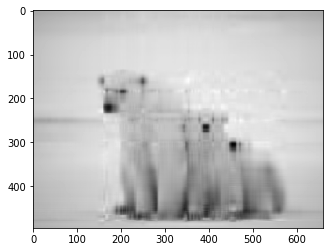
\includegraphics[scale = .35]{./polarbears_10sv.png}\\
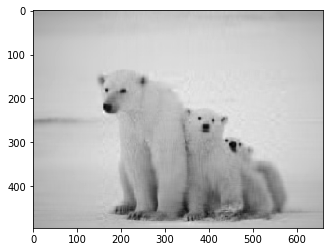
\includegraphics[scale = .35]{./polarbears_25sv.png}
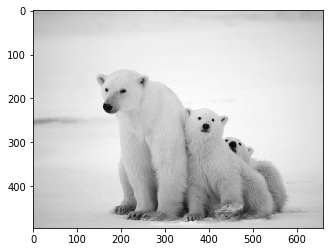
\includegraphics[scale = .35]{./polarbears_100sv.png}
\end{center}
\caption{The original  image is a $\rset^{495\times 660}$ matrix  of pixels (grey scale).   The image is then reconstructed using only the largest (top left), the first ten (top right), the first 25 (bottom left) and the first 100 (bottom right) singular values.}
\end{figure}
\end{frame}

\begin{frame}{Singular value decomposition}
\begin{figure}
\begin{center}
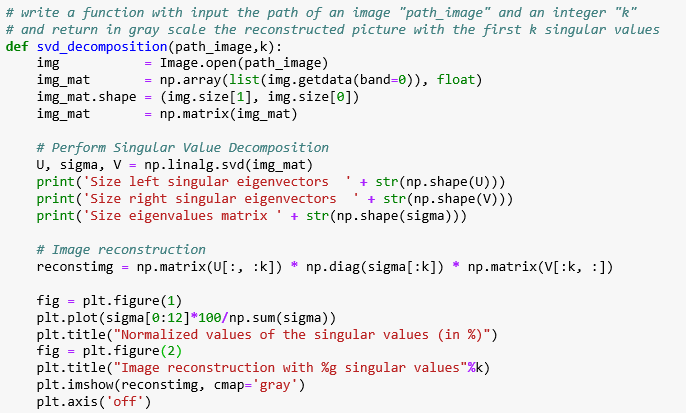
\includegraphics[scale = .45]{./svd_python.png}\\

\vspace{.2cm}

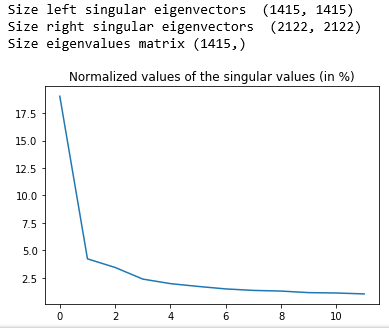
\includegraphics[scale = .35]{./svd_python_out1.png}
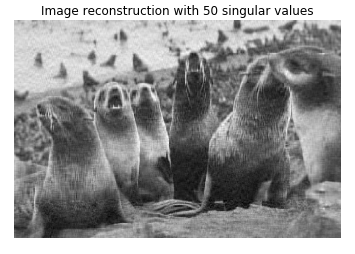
\includegraphics[scale = .35]{./svd_python_out2.png}
\end{center}
\end{figure}
\end{frame}

\section{Principal component analysis}

\begin{frame}{Principal component analysis}

\textcolor{lighto}{{\bf Principal component analysis}} is a multivariate technique which allows to analye the statistical structure of high dimensional dependent observations by representing data using \textcolor{lighto}{orthogonal variables called {\em principal components}}. 

\vspace{.3cm}
%Its origin may be traced back to \cite{hotelling:33} who first introduced the principal components as a way to reduce the dimensionality of the data. Reducing the dimensionality of the data is motivated by several practical reasons such as improving computational complexity.

Let $(X_i)_{1\leqslant i\leqslant n}$ be i.i.d. random variables in $\rset^d$ and consider the matrix $X\in\rset^{n\times d}$ such that the $i$-th row of $X$ is the observation $X^T_i$. 

\vspace{.3cm}

It is assumed that data are preprocessed so that \textcolor{violet}{the columns of $X$ are centered}.  This means that for all $1\leqslant p \leqslant d$, $\sum_{i=1}^{n}X_{i,k} = 0$. Let $\Sigma_n$ be \textcolor{violet}{the empirical covariance matrix}:
\begin{align*}
\Acolorboxed{\Sigma_n &= n^{-1}\sum_{i=1}^n X_i X^T_i\eqsp.}
\end{align*}

Note that \textcolor{lighto}{$\sum_{i=1}^n X_i X^T_i = X^TX$ so that $\Sigma_n = (X/\sqrt{n})^T(X/\sqrt{n})$} and \textcolor{violet}{the eigenvalue decomposition of $\Sigma_n$ allows to recover the singular values of $X/\sqrt{n}$ and its right-singular vectors}.
\end{frame}

%\begin{frame}
%\frametitle{}
%\vfill
%\begin{center}
%\blue{\huge{Principal Component Analysis} }
%\end{center}
%\vfill
%\begin{enumerate}
%\item Data - Issues - Preprocessing
%\item Observations Study
%\item Variables Study
%\item Interpretation Tools
%\end{enumerate}
%\end{frame}

%\section{Data - Issues}

\begin{frame}{PCA for which data?}

%PCA deals with continuous variables, but categorical ones can also be included 
%\vfill
%\begin{figure}
%\begin{minipage}{0.3\textwidth}
%\begin{figure}[H]
%\begin{center}
%\includegraphics[width=\textwidth]{fig/tabdon.pdf} \caption{Data table}
%\end{center}
%\end{figure}
%\end{minipage} \hfill
%%%%%%%%%%%%
%\begin{minipage}{0.65\textwidth}

$\rightharpoondown$ \textcolor{lighto}{{\bf Environmental data}}\\
{\em Waters - physico-chemical analyses, towns - temperature}.

$\rightharpoondown$  \textcolor{lighto}{{\bf Economy}}\\
{\em Countries - economic indicators}.

$\rightharpoondown$  \textcolor{lighto}{{\bf Biology}}\\
{\em Cheeses - microbiological analyses, tumors - genes expression}.

\vspace{.4cm}

\textcolor{violet}{{\bf Observations study}}\\ 
{\em Similarity between observations with respect to all the variables,  partition between observations}.

\textcolor{violet}{{\bf Variables study}}\\
{\em Linear relationships between variables, visualization of the correlation matrix, find synthetic variables}.

\textcolor{violet}{{\bf Link between the two studies}}\\ 
{\em Characterization of the groups of observations with variables, specific observations to understand links between variables}.

\end{frame}


%
%\begin{frame}
%\frametitle{Objectives}
%\vfill
%\begin{itemize}
%\item \red{Observations study:}\\ similarity between observations with respect to all the variables \\ partition between observations
%\vfill
%\item \maroon{Variables study:}\\ linear relationships between variables \\ visualization of the correlation matrix\\ find synthetic variables
%\vfill
%\item Link between the two studies:\\ characterization of the groups of observations with variables \\ specific observations to understand links between variables
%\end{itemize}
%\vfill
%\end{frame}


%\section{Observations study}

%\begin{frame}
%\frametitle{Preprocessing... (not an appropriate word?)}
%
%\vfill
%$\Rightarrow$ Similarity between observations: Euclidean distance
%\vfill
%\begin{itemize}
%\item Choosing \red{active} variables
%\begin{eqnarray*}
%d^2(i,i')&=&\red{\sum_{k=1}^{K}} (x_{ik}-x_{i'k})^2
%\end{eqnarray*}
%\item Variables are  centered
%\begin{eqnarray*}
%d^2(i,i')&=&\sum_{k=1}^{K} ((x_{ik}-\bar x_k -(x_{i'k}-\bar x_k))^2
%\end{eqnarray*}
%$x_{ik} \hookrightarrow x_{ik}-\bar x_k$\\
%\item Standardizing variables or not?
%\begin{eqnarray*}
%d^2(i,i')=\sum_{k=1}^K \red{\frac{1}{s_k^2}} (x_{ik}-x_{i'k})^2
%\end{eqnarray*}
%
%\end{itemize}
%\end{frame}
%
%\begin{frame}
%\frametitle{Wine data}
%\vfill
%\begin{itemize}
%\item Sensory descriptors as active: only these variables are used to define the dimensions
%\item Variables are (centered and) standardized
%\end{itemize}
%\vfill
%\begin{center}
%
%\begin{figure}[H]
%\begin{center}
%\includegraphics[width=0.9\textwidth]{fig/wine_tab_don.pdf} 
%\end{center}
%\end{figure}
%\end{center}
%\vfill
%\end{frame}

%\begin{frame}
%\frametitle{Observations cloud}
%\begin{figure}[H]
%\begin{center}
%\includegraphics[width=0.7\textwidth]{fig/oiseaux2.jpg}
%\end{center}
%\end{figure}
%\begin{itemize}
%\item Study the structure, \emph{i.e.} the shape of the cloud of observations\\
%\item Observations are in $\mathbb{R}^K$\\
%\end{itemize}
%\vfill
%\end{frame}

\begin{frame}{Fit the observations cloud}
Find the \textcolor{lighto}{subspace which best sums up the data}.

\begin{figure}[H]
\begin{center}

\includegraphics[scale=.3]{./cham3.pdf}
\caption{Camel vs dromedary? \tiny{(J.P. Fenelon})}
\end{center}
\end{figure}
\vfill
$\rightharpoondown$  Closest representation by \textcolor{violet}{projection}.

$\rightharpoondown$  Best representation of the diversity, \textcolor{violet}{variability of the observations}.

\end{frame}


\begin{frame}{Fit the observations cloud - a compressed sensing approach}

$\rightharpoondown$ \textcolor{lighto}{{\bf Reducing the dimensionality of the observations}} $(X_i)_{1\leqslant i \leqslant n}$ using a \textcolor{lighto}{{\em compression} matrix $W\in \rset^{p\times d}$} with $p\leqslant d$ so that for each $1\leqslant i \leqslant n$, $WX_i$ ia a low dimensional representation of $X_i$. 

\vspace{.2cm}

$\rightharpoondown$ The original observation may then be \textcolor{lighto}{partially recovered} using another matrix $U\in \rset^{d\times p}$. 

\vspace{.2cm}

$\rightharpoondown$ Principal Component Analysis  computes $U$ and $W$ using the \textcolor{violet}{{\bf least squares approach}}:
\begin{align*}
\Acolorboxed{(U_{\star},W_{\star}) \in \hspace{-0.5cm}\underset{(U,W)\in \rset^{d\times p}\times \rset^{p\times d}}{\mathrm{argmin}}& \;\sum_{i=1}^n\|X_i - UWX_i\|^2\eqsp,}
\end{align*}

\vspace{.2cm}

$\rightharpoondown$ Let $(U_{\star},W_{\star})\in \rset^{d\times p}\times \rset^{p\times d}$ be a solution. \textcolor{violet}{{\bf Then, the columns of $U_{\star}$ are orthonormal and $W_{\star} = U^T_{\star}$}}.

\end{frame}

\begin{frame}{Fit the observations cloud - a compressed sensing approach}

Principal Component Analysis  computes $U$ and $W$ using the \textcolor{violet}{{\bf least squares approach}}:
\begin{align*}
\Acolorboxed{U_{\star}\in \hspace{-0.5cm}\underset{U\in \rset^{d\times p}\eqsp; U^TU = I_p}{\mathrm{argmin}}& \;\sum_{i=1}^n\|X_i - UU^TX_i\|^2\eqsp,}
\end{align*}

\vspace{.2cm}

For all $U\in\rset^{d\times p}$ such that $U^TU = I_p$,
\begin{align*}
\textcolor{lighto}{\sum_{i=1}^n\|X_i - UU^TX_i\|^2} &=  \sum_{i=1}^n\|X_i\|^2 + \sum_{i=1}^nX^T_iUU^TX_i - 2\sum_{i=1}^nX^T_iUU^TX_i\eqsp,\\
&=  \sum_{i=1}^n\|X_i\|^2 - \sum_{i=1}^nX^T_iUU^TX_i\eqsp,\\
&=  \sum_{i=1}^n\|X_i\|^2 \textcolor{lighto}{- \mathrm{trace}(U^TXX^TU)}\eqsp.
\end{align*}
Therefore, solving the PCA problem boils down to computing
\begin{align*}
\Acolorboxed{U_{\star} \in \hspace{-0.5cm}\underset{U\in \rset^{d\times p}\eqsp,\eqsp U^TU = I_p}{\mathrm{argmax}} \hspace{-.4cm}&\{ \mathrm{trace}(U^T\textcolor{lighto}{\Sigma_n}U)\}\eqsp.}
\end{align*}

\end{frame}

\begin{frame}{Fit the observations cloud - a compressed sensing approach}

Let $\{\vartheta_1,\ldots,\vartheta_d\}$ be \textcolor{violet}{{\bf orthonormal eigenvectors associated with the eigenvalues $\lambda_1\geqslant \ldots \geqslant \lambda_d$ of $\Sigma_n$}}. Then a solution to the PCA problem is given by the matrix $U_{\star}$ with columns $\{\vartheta_1,\ldots,\vartheta_p\}$ and $W_{\star} = U^T_{\star}$.

\vspace{.5cm}

$\rightharpoondown$ Compute the matrix $\Sigma_n$, obtain its \textcolor{lighto}{eigenvectors sorted by eigenvalues}.

\vspace{.3cm}

$\rightharpoondown$ Build the matrices $U_{\star}$ and $W_{\star} = U^T_{\star}$.

\vspace{.3cm}

$\rightharpoondown$ \textcolor{lighto}{Compressed data} in $\rset^p$ given by \textcolor{lighto}{$W_{\star}X_i$} for all $1\leqslant i \leqslant n$.

\end{frame}

\begin{frame}{Fit the observations cloud - a projection approach}

For any dimension $1\leqslant p \leqslant  d$, let $\calF_d^p$ be the \textcolor{lighto}{set of all vector suspaces of $\rset^d$ with dimension $p$}.

\vspace{.5cm}

Define the  linear span $V_p$ as
\begin{align*}
\Acolorboxed{V_p \in \underset{V\in \calF_d^p}{\mathrm{argmin}}& \;\sum_{i=1}^n\|X_i - \pi_V(X_i)\|^2\eqsp,}
\end{align*}
where \textcolor{lighto}{$\pi_V$ is the orthogonal projection onto the linear span $V$}.

\vspace{.5cm}

For all $1\leqslant p \leqslant d$,  a solution  is given by \textcolor{lighto}{$V_p = \mathrm{span}\{v_1, \ldots, v_p\}$} where
\begin{align*}
\Acolorboxed{v_1 \in \underset{v\in \rset^d\,;\,\|v\|=1}{\mathrm{argmax}} \textcolor{violet}{\sum_{i=1}^n\langle X_i,v\rangle^2} \quad\mbox{and for}\;\;  k \geqslant p\;,\;\; v_k \in \underset{\substack{v\in \rset^d\,;\,\|v\|=1\,;\\ \textcolor{violet}{v\perp v_1,\ldots,v\perp v_{k-1}}}}{\mathrm{argmax}}&\textcolor{violet}{\sum_{i=1}^n\langle X_i,v\rangle^2}\eqsp. }
\end{align*}

$\rightharpoondown$  By induction, $\{\vartheta_1,\ldots,\vartheta_p\}$, the \textcolor{violet}{{\bf orthonormal eigenvectors associated with the eigenvalues $\lambda_1\geqslant \ldots \geqslant \lambda_p$ of $\Sigma_n$}}, are solutions to this problem.
\end{frame}


\begin{frame}{Fit the observations cloud - first dimension}
The \textcolor{lighto}{first dimension} is defined by
$$
v_1 \in \underset{v\in \rset^d\,;\,\|v\|=1}{\mathrm{argmax}} \textcolor{violet}{\sum_{i=1}^n\langle X_i,v\rangle^2} 
$$

\vspace{.3cm}

The \textcolor{lighto}{projection of each observation} on this dimension is
\begin{align*}
\Acolorboxed{\pi_{V_1}(X_i) &= \langle X_i,\vartheta_1\rangle \vartheta_1\eqsp.}
\end{align*}

\vspace{.3cm}

The \textcolor{lighto}{first principal component is the vector with $i$-th entry equal to the coordinate of $X_i$ in $V_1$}:
\begin{align*}
\Acolorboxed{c_1 &= X\vartheta_1\eqsp,\quad \pi_{V_1}(X_i) = c_1(i)\vartheta_1\eqsp.}
\end{align*}
%\begin{eqnarray*}
 %P_{u_1}(x_{i.})&=&u_1(u_1'u_1)^{-1}u_1'x_{i.} =  u_1 <x_{i.},u_1>\\
 %F_{i1} &=&<x_{i.},u_1>
%\end{eqnarray*}
%Minimize distance between obs and their projections \\
%Maximize the variance (inertia) of the projected data  
%The goal of PCA is to maximize the empirical variance of the derived variable z1 over
%choices of projection direction u,
%\begin{itemize}
%\item Find the first axis $u_1$, for which:
%$$u_1^{\star}=\operatorname*{arg\,max}_{u_1\in \mathbb{R}^K,~ \| u_1 \|_2^{2}=1} \frac{1}{I} \sum_{i=1}^{I} F_{i1}^2=\operatorname*{arg\,max}_{u_1\in \mathbb{R}^K,~ \| u_1 \|_2^{2}=1} \frac{1}{I} \sum_{i=1}^{I} (u_1'x_{i.})^2 $$
%$u_1$ \red{loadings} - $F_{.1}$ principal component (PC), \red{scores} \\
%$$\operatorname*{max}_{u_1\in \mathbb{R}^K,~ \| u_1 \|_2^{2}=1} u_1^{'} \left(\sum_{i=1}^{I}  \frac{1}{I} x_{i.}x_{i.}^{'}\right) u_1 = \frac{u_1^{'}X^{'}Xu_1}{I}$$

%$\Rightarrow$ $u_1^{\star}$ the first eigenvector of  the covariance matrix $S=\frac{X'X}{I}$ associated with the largest eigenvalue $\lambda_1$. $\mbox{var}(F_{.1}) = \lambda_1$
%$var(F_{.1})=var(Xu_1)=1/I\ u'_1X'Xu_1=u'_1Su_1 = \lambda_1 u'_1u_1=\lambda_1
%\end{itemize}
\end{frame}


\begin{frame}{Fit the observations cloud - first dimension}
\begin{figure}
\begin{center}
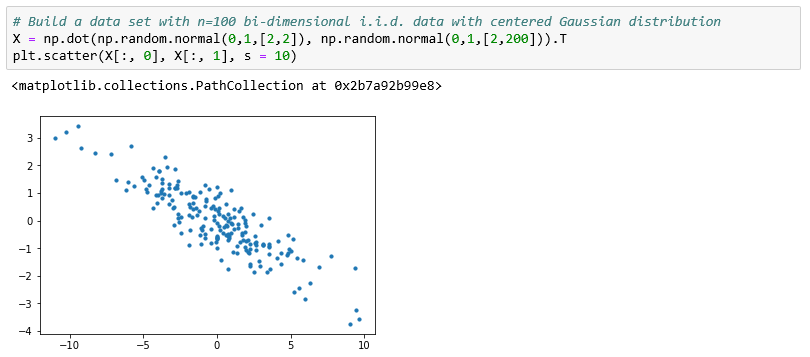
\includegraphics[scale = .55]{./pca_1comp_1.png}
\end{center}
\end{figure}
\end{frame}

\begin{frame}{Fit the observations cloud - first dimension}
\begin{figure}
\begin{center}
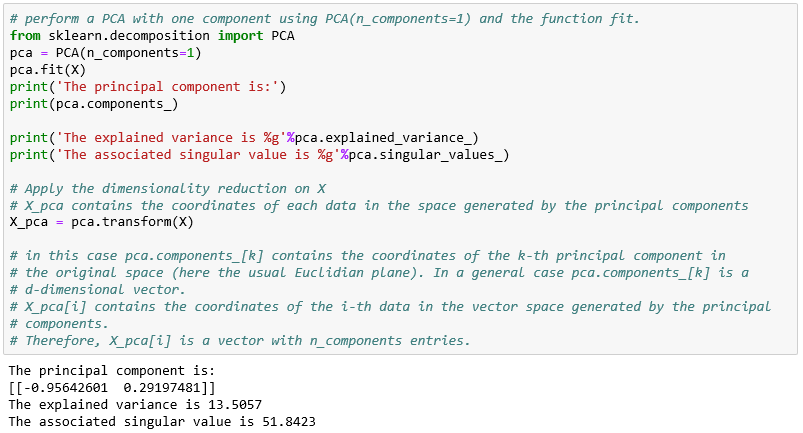
\includegraphics[scale = .55]{./pca_1comp_2.png}
\end{center}
\end{figure}
\end{frame}

\begin{frame}{Fit the observations cloud - first dimension}
\begin{figure}
\begin{center}
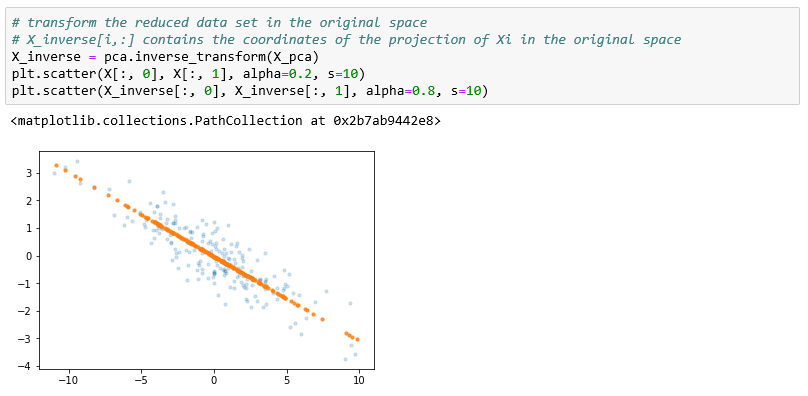
\includegraphics[scale = .55]{./pca_1comp_3.png}
\end{center}
\end{figure}
\end{frame}

\begin{frame}{Fit the observations cloud - additional dimensions}

As $V_p = \mathrm{span}\{\vartheta_1, \ldots, \vartheta_p\}$, for all $1\leqslant i\leqslant n$,
\begin{align*}
\Acolorboxed{\pi_{V_p}(X_i) &= \sum_{k=1}^p \langle X_i,\vartheta_k\rangle \vartheta_k  = \sum_{k=1}^p (X^T_i \vartheta_k)\vartheta_k = \sum_{k=1}^p c_k(i)\vartheta_k\eqsp,}
\end{align*}
where for all $1\leqslant k \leqslant p$, \textcolor{lighto}{the $k$-th principal component is defined as $c_k = X\vartheta_k$}.

\vspace{.2cm}

As already highlighted, \textcolor{lighto}{$U_*^TX_i$ contains the coordinates of $\pi_{V_p}(X_i) $ in  $V_p$}.

\vspace{.3cm}

\textcolor{violet}{{\bf Representation quality (dimensionality reduction loses information)}}

$\rightharpoondown$  \textcolor{lighto}{Total variance of the observations} (total inertia):
$$
\frac{1}{n} \sum_{i=1}^n \sum_{k=1}^d (X_{ik})^2 = \mathrm{trace}(\Sigma_n)= \sum_{k=1}^d \lambda_k\eqsp.
$$

$\rightharpoondown$ \textcolor{lighto}{Variance of the projected observations}  ($p$-dimensional representation):
$$
\mathrm{Var}(c_1) + \ldots + \mathrm{Var}(c_p) \eqsp.
$$

$\rightharpoondown$ \textcolor{lighto}{Percentage of inertia explained}: $\sum_{k=1}^{p} \lambda_k/\sum_{k=1}^{d} \lambda_k$.
\end{frame}

\begin{frame}{Fit the observations cloud - graphical representation}

The first principal component is  $c_1 = X\vartheta_1$ so that for aeach observation $1\leqslant i \leqslant n$, $c_1(i) = X^T_i\vartheta_1$.

$\rightharpoondown$ $\vartheta_1$ is also known as the \textcolor{lighto}{first loading vector}.

$\rightharpoondown$ $(c_1(i) = X^T_i\vartheta_1)_{1\leqslant i\leqslant n}$ are \textcolor{lighto}{the scores of the first principal component}.

\vspace{.3cm}

\textcolor{violet}{{\bf Application to the USArrests dataset}}\footnote{https://www.kaggle.com/deepakg/usarrests}

$\rightharpoondown$ Arrests per 100.000 residents for assault, murder and rape for the 50 US states in 1973. Percent of the population living in urban areas are also given.

\vspace{.1cm}

\begin{figure}[H]
\begin{center}
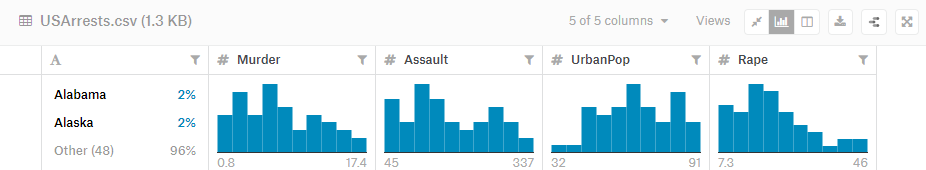
\includegraphics[scale=0.45]{usarrests} 
\end{center}
\end{figure}

\end{frame}


\begin{frame}{Fit the observations cloud - graphical representation}

{\small $\rightharpoondown$ Principal component \textcolor{lighto}{loading vectors $\vartheta_1$ and $\vartheta_2$}.}

\vspace{.1cm}

\begin{center}
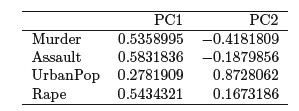
\includegraphics[scale=0.75]{usarrests_pc} 
\end{center}

In this setting \textcolor{lighto}{$n = 50$} (number states) and \textcolor{lighto}{$d = 4$} (number of variables - Murder, Assault, Rape and UrbanPop).

\begin{align*}
\vartheta_1 &= (0.53,0.58,0.28,0.54)\eqsp,\\
\vartheta_2 &= (-0.42,-0.19,0.87,0.17)\eqsp.
\end{align*}

%{\small $\rightharpoondown$ \textcolor{violet}{{\bf Biplot}\footnote{An introduction to statistical learning, {\bf James, G. and Witten, D. and Hastie, T. and Tibshirani, R.}, }}.}\\
%{\small States names in blue are the \textcolor{lighto}{the scores for the two first principal components $\vartheta_1$ and $\vartheta_2$} (coordinates of the projected observations).\\
%Orange arrows are  \textcolor{lighto}{the first two principal component loading vectors}.}
%
%\vspace{-.1cm}
%
%\begin{center}
%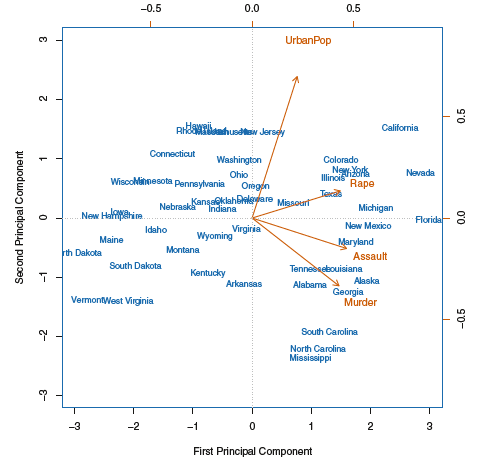
\includegraphics[scale=0.35]{biplot} 
%\end{center}

\end{frame}

\begin{frame}{Fit the observations cloud - graphical representation}

{\small $\rightharpoondown$ \textcolor{violet}{{\bf Biplot}\footnote{{\tiny An introduction to statistical learning, {\bf James, G. and Witten, D. and Hastie, T. and Tibshirani, R.}} }}.}\\
{\small States names in blue are the \textcolor{lighto}{the scores for the two first principal components} (coordinates of the projected observations).}

\vspace{-.5cm}

\begin{align*}
\Acolorboxed{\pi_{V_2}(X_i) &= (X_i^T\vartheta_1)\vartheta_1 + (X_i^T\vartheta_2)\vartheta_2\eqsp.}
\end{align*}

\begin{center}
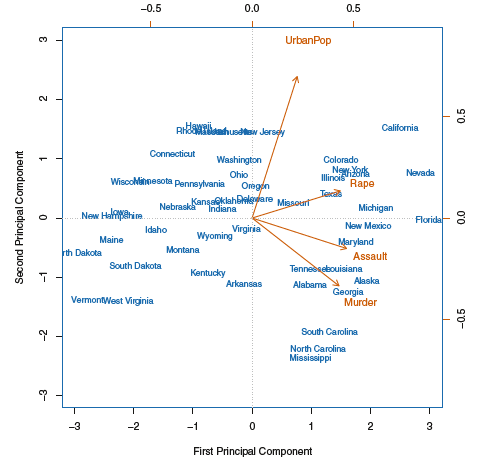
\includegraphics[scale=0.45]{biplot} 
\end{center}

\end{frame}

\begin{frame}{Fit the observations cloud - graphical representation}
 Let $W_p$ be the vector subspace of $\rset^n$ generated by $\{c_1,\ldots,c_p\}$. Since $(c_j)_{1 \leqslant j\leqslant d}$ form a orthogonal basis of $W_p$, for all $1\leqslant j\leqslant d$, 
\begin{align*}
\Acolorboxed{\pi_{W_p}(X_{.,j}) &= \sum_{\ell=1}^p \frac{\langle c_{\ell}, X_{.,j}\rangle }{\|c_{\ell}\|^2 }c_{\ell}\eqsp.}
\end{align*}

\vspace{.3cm}

As for all $1\leqslant \ell\leqslant d$, $\|c_{\ell}\|^2 = n \lambda_{\ell}$ and 
\begin{align*}
\Acolorboxed{\langle c_{\ell}, X_{.,j} \rangle  &= \langle X \vartheta_{\ell} , X_{.,j} \rangle  = X^T_{.,j}X\vartheta_{\ell} = (X^TX\vartheta_{\ell})_j = (n \Sigma_n \vartheta_{\ell})_j = n \lambda_{\ell} \vartheta_{\ell}(j)\eqsp.}
\end{align*}

\vspace{.3cm}

This yields, for all $1\leqslant j\leqslant d$, $\textcolor{lighto}{\pi_{W_p}(X_{.,j}) = \sum_{\ell=1}^p \vartheta_{\ell}(j)c_{\ell}}$.

\vspace{.3cm}

 $\rightharpoondown$ \textcolor{violet}{The coordinates of each variable $j$ in the space generated by the principal components are the loadings values} $(\vartheta_{\ell}(j))_{1\leqslant \ell\leqslant p}$.

 $\rightharpoondown$ \textcolor{violet}{The variables can be plotted as points in the component space using their loadings as coordinates.}
\end{frame}

\begin{frame}{Fit the observations cloud - graphical representation}

{\small $\rightharpoondown$ \textcolor{violet}{{\bf Biplot}\footnote{{\tiny An introduction to statistical learning, {\bf James, G. and Witten, D. and Hastie, T. and Tibshirani, R.}} }}.}\\
{\small Orange arrows are \textcolor{lighto}{the loadings for the two first principal components}.}

\vspace{-.5cm}

\begin{align*}
\Acolorboxed{\pi_{W_2}(X_{.,j}) &= \sum_{\ell=1}^2 \vartheta_{\ell}(j)c_{2}\eqsp.}
\end{align*}

\begin{center}
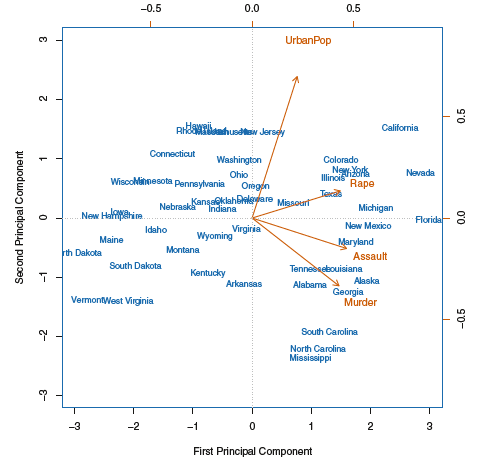
\includegraphics[scale=0.45]{biplot} 
\end{center}

\end{frame}

%\begin{frame}{$\mathrm{Cos}^2$ : quality of the representation for variables on the factor map}
%
%The sum of the cos2 for variables on the principal components is equal to one.
%
%If a variable is perfectly represented by only two components, the sum of the cos2 is equal to one. In this case the variables will be positioned on the circle of correlations.
%
%For some of the variables, more than 2 components are required to perfectly represent the data. In this case the variables are positioned inside the circle of correlations.
%
%
%The cos2 values are used to estimate the quality of the representation
%The closer a variable is to the circle of correlations, the better its representation on the factor map (and the more important it is to interpret these components)
%Variables that are closed to the center of the plot are less important for the first components.
%
%\end{frame}

%\begin{frame}
%\frametitle{Mean centring, Scaling?}
%\begin{itemize}
%\item Mean centring does not modify the shape of the cloud 
%\item Scaling is necessary when variables are not in the same units
%\end{itemize}
%\begin{figure}
%\begin{minipage}{0.45\textwidth}
%\includegraphics[scale=0.55]{fig/long_m.pdf}
%\end{minipage} \hfill
%%%%%%%%%%%%
%\begin{minipage}{0.45\textwidth}
%\includegraphics[scale=0.55]{fig/long_cm.pdf}
%\end{minipage}
%\end{figure}
%
%$\Rightarrow$ PCA always centred and often scaled 
%
%\end{frame}

%\begin{frame}{Fit the observations cloud - coordinates in the principal component space}
% For all $1\leqslant i\neq j \leqslant p$,
%$$
%\langle c_i,c_j\rangle = \vartheta'_i X' X \vartheta_j = \vartheta'_i(n\Sigma_n)\vartheta_j = n \lambda_j \vartheta'_i\vartheta_j = 0\eqsp, 
%$$
%as \textcolor{lighto}{$\{\vartheta_1, \ldots, \vartheta_d\}$ is an orthonormal family}. 
%
%\vspace{.3cm}
%
%Let $W_p$ be the vector subspace of $\rset^d$ \textcolor{lighto}{generated by $\{c_1,\ldots,c_p\}$}. Since $(c_j)_{1 \leqslant j\leqslant p}$ form a orthogonal basis of $W_d$, for all $1\leqslant i\leqslant n$, 
%\[
%\pi_{W_p}(X_i) = \sum_{j=1}^p \frac{\langle c_{j}, X_i\rangle }{\|c_{j}\|^2 }c_{j}\eqsp.
%\]
%For all $1\leqslant j\leqslant p$, \textcolor{lighto}{$\|c_{j}\|^2 = n \lambda_{j}$} and 
%\[
%\langle c_{j}, X_i \rangle  = \langle X \vartheta_{j} , X_i \rangle  = X_i'X\vartheta_{j} = (X'X\vartheta_{j})_i = (n \Sigma_n \vartheta_{j})_i = n \lambda_{j} \vartheta_{j}(i)\eqsp.
%\]
%This yields, for all $1\leqslant i\leqslant n$, 
%\[
%\textcolor{lighto}{\pi_{W_d}(X_i) = \sum_{j=1}^d \vartheta_{j}(i)c_{j}}\eqsp.
%\]
%\end{frame}



%\begin{frame}
%\frametitle{Wine: graph of observations}
%\vfill
%\begin{figure}[H]
%\begin{center}
%\includegraphics[width=0.65\textwidth]{fig/wine_PCA_ind}
%\end{center}
%\end{figure}
%$\Rightarrow$ Need variables to interpret the dimensions of variability
%\vfill
%\end{frame}

%\begin{frame}
%\frametitle{Observations coordinates considered as variables}
%\vfill
%\begin{figure}[H]
%\begin{center}
%\includegraphics[width=\textwidth]{fig/axe_composante.pdf} 
%\end{center}
%\end{figure}
%$F=Xu$ (linear combination of variables)
%\vfill
%\end{frame}

%\begin{frame}
%\frametitle{Interpretation of the observations graph with the variables}
%\vfill
%\begin{itemize}
%\item Correlation between variable $x_{.k}$ and $F_{.1}$ (and $F_{.2}$) 
%\vfill
%\begin{figure}[H]
%\begin{center}
%\includegraphics[scale=0.40]{fig/proj_1_var.pdf}
%\end{center}
%\end{figure}
%
%\vfill
%$\Rightarrow$ Correlation circle
%\vfill
%\end{itemize}
%\vfill
%\end{frame}

\begin{frame}{A classical example - wine data}

$\rightharpoondown$ \textcolor{violet}{{\bf 10 observations (rows)}}: white wines from Val de Loire.

$\rightharpoondown$ \textcolor{violet}{{\bf 30 variables (columns)}}:
\begin{enumerate}[-]
\item \textcolor{lighto}{27 continuous variables}: sensory descriptors.
\item \textcolor{lighto}{2 continuous variables}: odour and overall preferences.
\item \textcolor{lighto}{1 categorical variable}: label of the wines (Vouvray - Sauvignon).
\end{enumerate}

\begin{figure}[H]
\begin{center}
\includegraphics[width=\textwidth]{./wine_tab_don.pdf} 
\end{center}
\end{figure}
\vfill
\end{frame}

\begin{frame}
\frametitle{Interpretation of the observations graph with the variables}
\vfill
\begin{figure}[H]
\includegraphics[width=0.7\textwidth]{./wine_PCA_var.pdf}
\end{figure}
\vfill
\end{frame}
%
%\section{Variables study}
%
%\begin{frame}
%\frametitle{Cloud of variables}
%
%\begin{figure}
%\includegraphics[width=0.45\textwidth]{fig/nuage_var.pdf} 
%\end{figure}
%Inner product $<x_{.k},x_{.l}>_D = \frac{1}{I}\sum_{i=1}^I x_{ik}x_{il}$ induces correspondence between geometry and statistics. $D$ diag matrix with $1/I$
%$$cos(\theta_{kl})=\frac{<x_{.k},x_{.l}>_D}{\|x_{.k}\|_D\ \|x_{.l}\|_D}=\frac{\sum_{i=1}^I x_{ik}x_{il}}{\sqrt{(\sum_{i=1}^I x_{ik}^2)(\sum_{i=1}^I x_{il}^2)}}=r(x_{.k},x_{.l})$$
%\vfill
%\end{frame}
%
%\begin{frame}
%\frametitle{Fit the variables cloud}
%
%Find $v_1$ (in $\mathbb{R}^I$, with $v_1'Dv_1=1$) which best fits the cloud
%\begin{figure}
%\begin{minipage}{0.45\textwidth}
%\includegraphics[scale=0.55]{fig/proj_var.pdf} 
%\end{minipage} \hfill
%%%%%%%%%%%%
%\begin{minipage}{0.45\textwidth}
%\begin{eqnarray*}
% P_{v_1}(x_{.k})&=&v_1(v_1'Dv_1)^{-1}v_1'Dx_{.k}\\
% G_{k1} &=&  <x{.k}, v_1>_D \\
% G_{k1} &=& \frac{<v_1,x{.k}>_D}{\|v_1\|_D\ \|x_{.k}\|_D}
%\end{eqnarray*}
%\end{minipage}
%\end{figure}
%\vfill
%$$\operatorname*{arg\,max}_{v_1\in \mathbb{R}^I, ~  \|v_{1}\|_D^{2}=1} \sum_{i=k}^K G_{k1}^2 = \red{\operatorname*{arg\,max}_{v_1\in \mathbb{R}^I, ~  \|v_{1}\|_D^{2}=1} \sum_{i=k}^K r(v_1,x_{.k})^2} $$
%\vfill
%$\Rightarrow$ $v_1$ is the best synthetic variable
%\vfill
%$\Rightarrow$ $v_1, ...,v_Q$ are eigenvectors of $WD=XX'D$  associated with the largest eigenvalues:
%$WDv_q=\lambda_q v_q$
%\vfill
%\end{frame}

%
%\begin{frame}
%\frametitle{Fit the variables cloud}
%\vfill
%\begin{figure}[H]
%\begin{center}
%\includegraphics[width=0.7\textwidth]{fig/wine_PCA_var.pdf}
%\end{center}
%\end{figure}
%$\Rightarrow$ Same representation
%\vfill
%\end{frame}
%
%\begin{frame}
%\frametitle{Projections...}
%
%\vfill
%$ r(x_{.1},x_{.2}) = cos(\theta_{x_{.1},x_{.2}})$\\
%$ cos(\theta_{x_{.1},x_{.2}}) \approx cos(\theta_{H_1,H_2}) $ if variables are well projected
%
%\begin{figure}[H]
%\begin{center}
%\includegraphics[scale=0.35]{fig/proj_var_acp.pdf}
%\end{center}
%\end{figure}
%\vfill
%Only well projected variables can be interpreted
%\vfill
%\end{frame}

%\begin{frame}
%\frametitle{Link between the two representations: transition formulae}
%\begin{figure}[H]
%\begin{center}
%\includegraphics[width=0.72\textwidth]{fig/link.pdf}
%\end{center}
%\end{figure}
%\end{frame}
%
%
%\begin{frame}
%\frametitle{Link between the two representations: transition formulae}
%\vfill
%\begin{itemize}
%\item $Su= (1/I)X'Xu=\lambda u$ \\
%\item $XX'DXu=X\lambda u$ $\rightarrow$ $WD(Xu)= \lambda (X u) $\\
%\item $WDF=\lambda F$ and $ WDv=\lambda v$: $F$ and $v$ are collinear\\
%\item \red{$||F||_D^2=\lambda$} and $||v||_D^2= 1$: \\
%\end{itemize}
%\begin{center}
%\begin{tabular}{lll}
%&\red{$v= \frac{1}{\sqrt{\lambda}} F$}   &  $\Rightarrow$
%$G=X'Dv= \frac{1}{\sqrt{\lambda}}X'DF$\\
%& $u=\frac{1}{\sqrt{\lambda}}G$ &
%$\Rightarrow$  $F=Xu=\frac{1}{\sqrt{\lambda}}XG$ \\
%\end{tabular}
%\vfill
%\begin{tabular}{cc}
%$\boxed{F_{iq}=\frac{1}{\sqrt{\lambda_q}}\sum_{k=1}^K x_{ik}G_{kq}}$ & $\boxed{G_{kq}=\frac{1}{\sqrt{\lambda_q}}\sum_{i=1}^I (1/I) x_{ik}F_{iq}}$\\
%\end{tabular}
%\end{center}
%$F_{.q}$: principal components (variance=eigenvalues), scores\\
%$G_{.q}$: correlations between variables and principal components
%\vfill
%\end{frame}
%
%\begin{frame}
%\frametitle{Link between the two representations: transition formulae}
%\vfill
%\begin{center}
%\begin{tabular}{cc}
%$\boxed{F_{iq}=\frac{1}{\sqrt{\lambda_q}}\sum_{k=1}^K x_{ik}G_{kq}}$ & $\boxed{G_{kq}=\frac{1}{\sqrt{\lambda_q}}\sum_{i=1}^I (1/I)x_{ik}F_{iq}}$\\
%\end{tabular}
%\end{center}
%\vfill
%Observation on the side of the variables where it takes high values
%\begin{figure}[H]
%\begin{tabular}{ll}
%\includegraphics[width=0.4\textwidth]{fig/wine_PCA_ind}&\includegraphics[width=0.6\textwidth]{fig/wine_PCA_var.pdf}\\
%\end{tabular}
%\caption{observations and variables representations}
%\end{figure}
%\end{frame}
%
%\section{Interpretation tools}

\begin{frame}{Supplementary information}

\begin{enumerate}[-]
\item Supplementary variables \textcolor{lighto}{do not impact PCA results} but may provide insights on their interpretability.
\item In R, supplementary continuous variables added by \textcolor{lighto}{quanti.sup} and discrete variables added with \textcolor{lighto}{quali.sup}.
\item In the case of discrete variables,  the \textcolor{lighto}{barycentre of the observations which take each category} is displayed in the observations plot.

\begin{center}
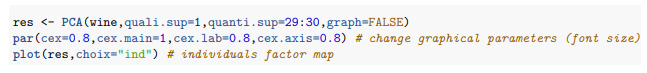
\includegraphics[width=0.65\textwidth]{pca_supp_1}\\
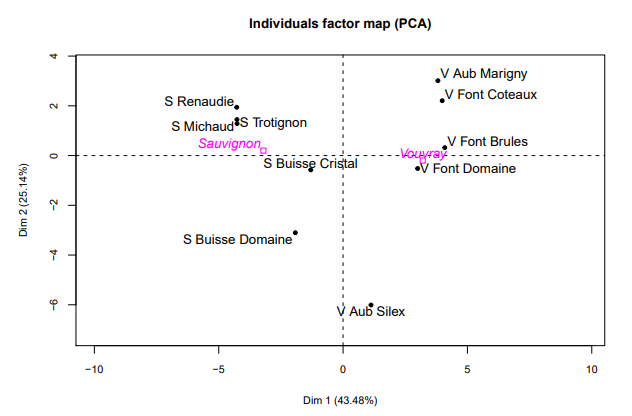
\includegraphics[width=0.65\textwidth]{pca_supp_2}
\end{center}

\end{enumerate}

\end{frame}

\begin{frame}{Supplementary information}

\begin{enumerate}[-]

\item In the case of continuous variables,  \textcolor{lighto}{additional variables are projected in the factor map}.

\begin{center}
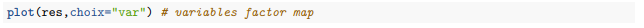
\includegraphics[width=0.65\textwidth]{pca_supp_3}\\
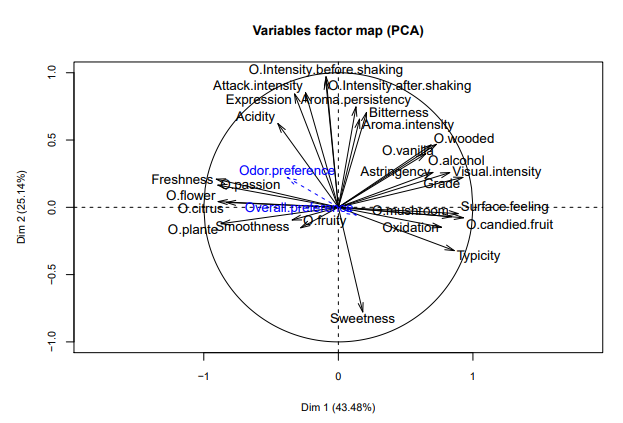
\includegraphics[width=0.65\textwidth]{pca_supp_4}
\end{center}

\end{enumerate}

\end{frame}

\begin{frame}{Supplementary information}

\begin{enumerate}[-]

\item Drawing with a color  \textcolor{lighto}{according to the label}.

\begin{center}
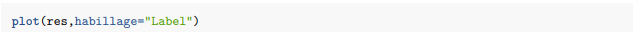
\includegraphics[width=0.65\textwidth]{pca_supp_5}\\
\includegraphics[width=0.65\textwidth]{./wine_PCA_ind_mod_coul.pdf}
\end{center}

\end{enumerate}

\end{frame}

\begin{frame}{Choosing the number of components}

$\rightharpoondown$ The problem is to figure out \textcolor{lighto}{which amount of information} should be extracted from the original dataset. \textcolor{lighto}{{\bf How many components need to be considered?}}

$\rightharpoondown$ Open problem for which a \textcolor{lighto}{few practical guidelines exist}.

$\rightharpoondown$  \textcolor{violet}{{\bf Bar plot for illustrative purposes}}.

\begin{center}
\includegraphics[width=.5\textwidth]{./wine_pca_eig.pdf}
\end{center}

\end{frame}


\begin{frame}{Choosing the number of components}

$\rightharpoondown$ A \textcolor{lighto}{scree plot} may be used to  plot the eigenvalues according to their size.

$\rightharpoondown$ \textcolor{lighto}{Detect the elbow}, i.e. the eigenvalue where the \textcolor{lighto}{slope in this graph goes from
steep to flat}:  keep only the components which are before the elbow.  

\begin{center}
\includegraphics[width=.75\textwidth]{./screeplot}
\end{center}

\end{frame}


\begin{frame}{Choosing the number of components - going further}

$\rightharpoondown$  \textcolor{lighto}{estim\_ncpPCA} may be used to  estimate the number of components using cross validation.

\vspace{.2cm}

$\rightharpoondown$ In the default case, \textcolor{lighto}{leave-one-out} cross validation, each value $X_{ik}$ \textcolor{lighto}{is iteratively removed from the dataset}. This value is then estimated by $\widehat{X}^r_{ik}$ using a PCA with $r$ components obtained from the dataset that excludes this cell (with \textcolor{lighto}{imputePCA}).

\vspace{.2cm}

$\rightharpoondown$ The estimated number of components is then
\begin{align*}
\Acolorboxed{& r\mapsto \frac{1}{nd}\sum_{i=1}^{n}\sum_{k=1}^{d}\left(X_{ik}-\widehat{X}^r_{ik}\right)^2\eqsp.}
\end{align*}

\vspace{.2cm}

$\rightharpoondown$ \textcolor{lighto}{$K$-fold cross validation} is also possible with a given proportion of data to be removed.


\end{frame}

%\begin{frame}{Quality of the representation: $\cos^2(\theta)$}
%\vfill
%$\Rightarrow$ Projected inertia of  an element / total inertia of the element
%\vfill
%\begin{itemize}
%\item observations: $\frac{F_{iq}^2}{d^2(x_{i.},G_I)} = \frac{F_{iq}^2}{\sum_{q=1}^K F_{iq}^2} $ 
%\begin{scriptsize}
%\begin{verbatim}
%round(res.pca$ind$cos2,2)
%                 Dim.1 Dim.2
%S Michaud         0.62  0.07
%S Renaudie        0.73  0.15
%S Trotignon       0.78  0.07
%\end{verbatim}
%\end{scriptsize}
%\vfill
%\item variables: squared coordinate
%\begin{scriptsize}
%\begin{verbatim}
%round(res.pca$var$cos2,2)
%                              Dim.1 Dim.2 
%Odor.Intensity.before.shaking  0.01  0.94 
%Odor.Intensity.after.shaking   0.01  0.89 
%Expression                     0.11  0.71 
%\end{verbatim}
%\end{scriptsize}
%\end{itemize}
%\vfill
%$\Rightarrow$ Only well projected elements can be interpreted
%
%\end{frame}


\begin{frame}{Contribution}

$\rightharpoondown$ \textcolor{lighto}{Contribution of an observation to the dimension $k$} (percentage of variability).

\begin{align*}
\Acolorboxed{& \mbox{Ctr}_k(X_{i}) =\frac{c_k(i)^2/n}{\sum_{i=1}^nc_{k}(i)^2/n}= \frac{c_{k}(i)^2}{n\lambda_k}\eqsp.}
\end{align*}

\begin{center}
\includegraphics[width=.5\textwidth]{./contrib}
\end{center}


$\rightharpoondown$ Observations with large coordinate contribute the most.
%\vfill
%\begin{scriptsize}
%\begin{verbatim}
%round(res.pca$ind$contrib,2)
%                 Dim.1 Dim.2 
%S Michaud        15.49  3.10 
%S Renaudie       15.56  5.56 
%S Trotignon      15.46  2.43 
%\end{verbatim}
%\end{scriptsize}
%\vfill
%\item variables: $\mbox{Ctr}_q(x_{k.}) = \frac{G_{kq}^2}{\lambda_q} = \frac{r(x_{.k},v_q)^2}{\lambda_q} $
%\vfill
%$\Rightarrow$ variables with large correlation contribute the most
%\vfill
%\end{itemize}
\end{frame}

%\begin{frame}[fragile]
%\frametitle{Description of  dimensions}
%\vfill
%\vfill
%Using continuous variables:
%\begin{itemize}
%\item correlation between variable and the principal components
%\item sort correlation coefficients and give significant ones (rought tests)
%\end{itemize}
%
%\begin{scriptsize}
%\begin{verbatim}
%> dimdesc(res.pca)
%
%   			        $Dim.1$quanti                               $Dim.2$quanti
%                 corr p.value                                corr p.value
%O.candied.fruit  0.93 9.5e-05  Odor.Intensity.before.shaking 0.97 3.1e-06
%Grade            0.93 1.2e-04  Odor.Intensity.after.shaking  0.95 3.6e-05
%Surface.feeling  0.89 5.5e-04  Attack.intensity              0.85 1.7e-03
%Typicity         0.86 1.4e-03  Expression                    0.84 2.2e-03
%O.mushroom       0.84 2.3e-03  Aroma.persistency             0.75 1.3e-02
%Visual.intensity 0.83 3.1e-03  Bitterness                    0.71 2.3e-02
%   ...            ...     ...  Aroma.intensity               0.66 4.0e-02
%O.plante        -0.87 1.0e-03
%O.flower        -0.89 4.9e-04
%O.passion       -0.90 4.5e-04
%Freshness       -0.91 2.9e-04  Sweetness                    -0.78 8.0e-03
%\end{verbatim}
%\end{scriptsize}
%
%\end{frame}
%
%\begin{frame}[fragile]
%\frametitle{Description of dimensions}
%\vfill
%Using categorical variables:\\
%\begin{itemize}
%\item One-way anova with the coordinates of
%   the observations ($F_{.q}$) explained by the categorical variable
%\begin{itemize}
%\item F-test by variable
%\item for each category, a Student's $T$-test to compare the average of the category with the general mean
%\end{itemize}
%\end{itemize}
%\begin{scriptsize}
%\begin{verbatim}
%> dimdesc(res.pca)
%
%Dim.1$quali
%             R2      p.value
%Label     0.874     7.30e-05
%
%Dim.1$category
%           Estimate      p.value
%Vouvray       3.203     7.30e-05
%Sauvignon    -3.203     7.30e-05
%\end{verbatim}
%\end{scriptsize}
%\end{frame}

\section{Kernel principal component analysis}

\begin{frame}{Kernel PCA}
$\rightharpoondown$ PCA only allows dimensionality reduction based on principal components which are \textcolor{lighto}{linear combinations of the variables}.


$\rightharpoondown$  When the data has more complex structures \textcolor{lighto}{which cannot be well represented in a linear
subspace}, standard PCA fails. 

$\rightharpoondown$  kernel PCA\footnote{{\tiny Kernel principal component analysis, {\bf Scholkopf, B. et al.}, {\em International Conference on Artificial Neural Networks}, p. 583-588, 1997}} allows us to generalize standard PCA to \textcolor{lighto}{nonlinear dimensionality reduction} (Scholkopf et al., 1999)\footnote{{\tiny Advances in kernel methods: support vector learning, {\bf Scholkopf et al.}, {\em MIT Press}}}.

\vspace{.3cm}

A function $k:\rset^d\times\rset^d:\to \rset$ is said to be a \textcolor{violet}{{\bf positive definite kernel}} if and only if it is symmetric and if for all $n\geqslant 1$, $(x_1,\ldots,x_n)\in(\rset^d)^n$ and all $(a_1,\ldots,a_n)\in\rset^n$,
\begin{align*}
\Acolorboxed{&\sum_{1\leqslant i,j\leqslant n}a_ia_jk(x_i,x_j) \geqslant 0\eqsp.}
\end{align*}
\end{frame}

\begin{frame}{Kernel PCA}
$\rightharpoondown$ Each observation $X_i$ is mapped into a \textcolor{lighto}{$m$-dimensional space using a function $\varphi: \rset^d\to\rset^m$}.


$\rightharpoondown$  The new features are assumed \textcolor{lighto}{to be centered}:
\begin{align*}
\Acolorboxed{&\sum_{i=1}^n\varphi(X_i) = 0\eqsp.}
\end{align*}

$\rightharpoondown$  The \textcolor{lighto}{covariance matrix of the new features} is
\begin{align*}
\Acolorboxed{&\Sigma_n = \frac{1}{n}\sum_{i=1}^n\varphi(X_i)(\varphi(X_i))^T\eqsp.}
\end{align*}

\vspace{.3cm}

Let $\vartheta_k$ be the eigenvectors of $\Sigma_n$ associated with the eigenvalues $\lambda_1\geqslant \lambda_2 \geqslant \ldots \geqslant \lambda_m$:
\begin{align*}
\Acolorboxed{&\Sigma_n \vartheta_k = \lambda_k \vartheta_k\eqsp.}
\end{align*}
\end{frame}

\begin{frame}{Kernel PCA}
$\rightharpoondown$ For each eigenvector $\vartheta_k$, there exist $(\alpha_{ki})_{1\leqslant i\leqslant n}$ such that

\begin{align*}
\Acolorboxed{&\vartheta_k = \sum_{i=1}^n \alpha_{ki}\varphi(X_i)\eqsp.}
\end{align*}

 This yields

\begin{align*}
\Acolorboxed{&\frac{1}{n}\sum_{i=1}^n\varphi(X_i)(\varphi(X_i))^T\left( \sum_{j=1}^n \alpha_{kj}\varphi(X_j)\right) = \lambda_k  \sum_{i=1}^n \alpha_{ki}\varphi(X_i)\eqsp.}
\end{align*}

$\rightharpoondown$  Defining \textcolor{lighto}{the kernel $\kappa(X_i,X_j) = (\varphi(X_i))^T\varphi(X_j))$}, for all $1\leqslant p \leqslant n$,
\begin{align*}
\Acolorboxed{&\frac{1}{n}\sum_{i=1}^n\sum_{j=1}^n \alpha_{kj}\kappa(X_p,X_i) \kappa(X_i,X_j) = \lambda_k  \sum_{i=1}^n \alpha_{ki}\kappa(X_p,X_i) \eqsp.}
\end{align*}

$\rightharpoondown$  Let $\mathsf{K}$ be the matrix defined as \textcolor{lighto}{$\mathsf{K}_{ij} =\kappa(X_i,X_j) = (\varphi(X_i))^T\varphi(X_j))$} and ${\bar \alpha}_k$ be the column vector with entries $(\alpha_{ki})_{1\leqslant i\leqslant n}$, so that,
\begin{align*}
\Acolorboxed{&\mathsf{K}^2\bar\alpha_{k} = n \lambda_k K\bar\alpha_{k}\eqsp.}
\end{align*}

\end{frame}

\begin{frame}{Kernel PCA}

$\rightharpoondown$  Only requires to compute \textcolor{lighto}{$\mathsf{K}_{ij} =\kappa(X_i,X_j) = (\varphi(X_i))^T\varphi(X_j))$}, to find the vector $\bar \alpha_k$ associated with the nonzero eigenvalue $\lambda_k$ such that
\begin{align*}
\Acolorboxed{&\mathsf{K} \bar\alpha_{k}= n \lambda_k \bar\alpha_{k}\eqsp.}
\end{align*}


$\rightharpoondown$ \textcolor{lighto}{Principal components} given by
\begin{align*}
\Acolorboxed{c_k(i) &= \varphi(X_i)^T\vartheta_k = \sum_{j=1}^n \alpha_{jk}K(X_i,X_j)\eqsp.}
\end{align*}
\textcolor{violet}{{\bf No need to evaluate $\varphi(X_i)$, only the kernel matrix is necessary}}.

$\rightharpoondown$ \textcolor{lighto}{If the new features are not centered}, the matrix $\mathsf{K}$ may be replaced by
\begin{align*}
\Acolorboxed{\widetilde{\mathsf{K}} &= 1_n\mathsf{K} - \mathsf{K}1_n + 1_n\mathsf{K}1_n\eqsp,}
\end{align*}
where $1_n$ is the $n\times n$ matrix with all elements equal to $1/n$.

\end{frame}

\begin{frame}{Kernel PCA in practice}

$\rightharpoondown$  \textcolor{violet}{{\bf Compute the kernel matrix $\mathsf{K}$}}, for instance based on the Gaussian radial basis function:
\begin{align*}
\Acolorboxed{&\mathsf{K}(X_i,X_j) = \mathrm{exp}\left(-\gamma\|X_i-X_j\|^2\right)\eqsp.}
\end{align*}

$\rightharpoondown$ \textcolor{lighto}{If the new features are not centered}, the matrix $\mathsf{K}$ may be replaced by
\begin{align*}
\Acolorboxed{\widetilde{\mathsf{K}} &= 1_n\mathsf{K} - \mathsf{K}1_n + 1_n\mathsf{K}1_n\eqsp.}
\end{align*}

$\rightharpoondown$ \textcolor{violet}{{\bf Compute the vector $\bar \alpha_k$}} by solving 
\begin{align*}
\Acolorboxed{&\mathsf{K} \bar\alpha_{k}= n \lambda_k \bar\alpha_{k}\eqsp.}
\end{align*}

$\rightharpoondown$ \textcolor{violet}{{\bf Compute the principal components}}: 
\begin{align*}
\Acolorboxed{c_k(i) &= \varphi(X_i)^T\vartheta_k = \sum_{j=1}^n \alpha_{jk}K(X_i,X_j)\eqsp.}
\end{align*}

\end{frame}

\begin{frame}{Kernel PCA in practice}

\begin{center}
\includegraphics[width = .8\linewidth]{./half_moon_1.png}
\includegraphics[width = .8\linewidth]{./half_moon_2.png}
\end{center}

\end{frame}

\begin{frame}{Kernel PCA in practice}

\begin{center}
\includegraphics[width = .8\linewidth]{./half_moon_3.png}
\end{center}

\end{frame}

\begin{frame}{Kernel PCA in practice}

\begin{center}
\includegraphics[width = .8\linewidth]{./half_moon_4.png}
\end{center}

\end{frame}

\begin{frame}{Kernel PCA in practice}

\begin{center}
\includegraphics[width = .8\linewidth]{./half_moon_5.png}
\end{center}

\end{frame}

\begin{frame}{Kernel PCA in practice}

\begin{center}
\includegraphics[width = .8\linewidth]{./half_moon_6.png}
\end{center}

\end{frame}

\section{Independent component analysis}

\begin{frame}{Linear independent component analysis}
$\rightharpoondown$ {\bf \textcolor{violet}{Linear independent component analysis}} of a random vector $X$ amounts to estimating the following model
\begin{align*}
\Acolorboxed{& X = AS + \varepsilon\eqsp,}
\end{align*}
where $A\in\rset^{d\times n}$ is an unknown \alert{mixing} matrix, $S\in\rset^{n}$ is a random vector with independent entries and $\varepsilon$ is an independent noise.

$\rightharpoondown$ Noise free formulation of this problem, i.e. $X = AS$, was proposed in the signal processing litterature\footnote{{\tiny Blind separation of sources, part I: an adaptive algorithm based on neuromimetic architecture. {\bf Jutten, C. et al.}, {\em Signal Processing, 2(4), 1-10}}, 1991}
\end{frame}

\begin{frame}{Linear independent component analysis - identifiability}
The {\bf \textcolor{violet}{noise free linear independent component analysis}} is identifiable under the following (sufficient conditions).

$\rightharpoondown$ 

\vspace{.3cm}

$\rightharpoondown$ 

\vspace{.3cm}

$\rightharpoondown$ 
\end{frame}

\section{Correspondence analysis}

\begin{frame}{Correspondence analysis}
$\rightharpoondown$ Similar to principal component analysis, \textcolor{lighto}{but applied to categorical data}. 


$\rightharpoondown$  Let $X$ be a $n\times d$ \textcolor{lighto}{contingency matrix}, i.e. a matrix of nonnegative integers. 

$\rightharpoondown$  The \textcolor{lighto}{correspondence matrix} is then 

\begin{align*}
\Acolorboxed{& P = (1_n^TX1_d)^{-1}X\eqsp,}
\end{align*}
where $1_n^TX1_d$ is the \textcolor{lighto}{total number of counts}.

$\rightharpoondown$ Principal components obtained by the \textcolor{lighto}{singular value decomposition of the standardized residuals}:
\begin{align*}
\Acolorboxed{& \Sigma = \mathrm{diag}(P1_d)^{-1/2}\left(P - P1_d1_n^TP\right)\mathrm{diag}(P^T1_n)^{-1/2}\eqsp.}
\end{align*}


\end{frame}

%\section{Multiple correspondence analysis}
%
%\section{Multiple factor analysis}
%





\begin{frame}{Other dimensionality reduction techniques}

$\rightharpoondown$  \textcolor{lighto}{Independent component analysis} (ICA)\footnote{{\tiny Independent component analysis: algorithms and applications, {\bf Hyvarinen, A. et al.}, {\em Neural networks, 13(4-5), 411-430}}, 2000}.

\vspace{.3cm}

$\rightharpoondown$ \textcolor{lighto}{Locally linear embedding} (LLE)\footnote{{\tiny Nonlinear dimensionality reduction by locally linear embedding, {\bf Row, S.T. et al.}, {\em Science, 290(5500), 2323-2326}}, 2000}.

\vspace{.3cm}

$\rightharpoondown$ \textcolor{lighto}{Uniform manifold approximation} (UMA)\footnote{{\tiny Umap: Uniform manifold approximation and projection for dimension reduction, {\bf McInnes, L. et al.}, {\em  arXiv:1802.03426}}, 2018}.

\vspace{.3cm}

$\rightharpoondown$ \textcolor{lighto}{Random forests}\footnote{{\tiny Random forests, {\bf Breiman, L. et al.}, {\em Machine learning, 45(1), 5-32}}, 2001}.

\end{frame}




%\begin{frame}[fragile]
%\frametitle{Practice with R}
%\vfill
%\begin{enumerate}
%\item Select active variables
%\item Scale or not the variables
%\item Perform PCA
%\item Choose the number of dimensions to interpret 
%\item Simultaneously interpret the observations and variables graphs
%\item Use interpretation tools
%\end{enumerate}
%\vfill
%\begin{scriptsize}
%\begin{verbatim}
%library(FactoMineR)
%Expert <- read.table("http://factominer.free.fr/course/doc/data_PCA_ExpertWine.csv",
%   header = TRUE, sep = ";", row.names = 1)
%res.pca <- PCA(Expert, scale = T, quanti.sup = 29:30, quali.sup = 1)
%summary(res.pca)
%barplot(res.pca$eig[,1], main = "Eigenvalues", names.arg = 1:nrow(res.pca$eig))
%plot.PCA(res.pca, habillage = 1)
%res.pca$ind$coord; res.pca$ind$cos2; res.pca$ind$contrib
%plot.PCA(res.pca, axes = c(3, 4), habillage = 1)
%dimdesc(res.pca)
%plotellipses(res.pca, 1)
%write.infile(res.pca, file = "my_FactoMineR_results.csv") 
%\end{verbatim}
%\end{scriptsize}
%\end{frame}
%
%%\begin{frame}[fragile]
%%\frametitle{References  PCA}
%%\vfill
%%Jolliffe (2002): PCA Springer
%%\vfill
%%\maroon{\href{http://web.stanford.edu/class/bios221/book/Chap-Multivariate.html}{Multivariate Analysis - Susan Holmes} }
%%\vfill
%%
%%\tiny{\maroon{\href{http://www.stat.rice.edu/~gallen/gallen_gmd.pdf}{A Generalized Least Squares Matrix Decomposition, Allen G. \textit{et al.} JASA (2014)}
%%\vfill
%%\href{http://statweb.stanford.edu/~susan/papers/dfc.pdf}{Multivariate Data Analysis: The French Way (S. Holmes)} }}
%%\vfill
%%
%%
%%
%%\end{frame}
%%
%%\begin{frame}[fragile]
%%\frametitle{References FactoMineR}
%%\begin{minipage}{0.4\textwidth}
%%\includegraphics[height=0.3\textheight]{fig/livre_anado_gb_2} \includegraphics[height=0.3\textheight]{fig/mfa} 
%%\end{minipage}~~
%%%%%%%%%%%%%
%%\begin{minipage}{0.6\textwidth}
%%\maroon{\emph{Exploratory Multivariate Analysis by Example using R}, Husson, Le, Pages  (2017),
%%Chapman \&  Hall \\  
%%\emph{Multiple Factor Analysis by Example using R}, Pages  (2015),
%%CRC Press}
%%\end{minipage}
%%\vfill
%%Package \texttt{FactoMineR}:
%%\maroon{\url{http://factominer.free.fr}}\\
%%Youtube:
%%\maroon{\href{https://www.youtube.com/playlist?list=PLnZgp6epRBbTsZEFXi_p6W48HhNyqwxIu}{playlist}}
%%\vfill
%%Packages - code: ade4, prcomp, pricomp \\
%%
%%\end{frame}
%%
%%\frame
%%%%%%%%%%%%%%%%%%%%%%%%%
%%{ \frametitle{Degustation}
%%\begin{center}
%%\includegraphics[width=0.9 \textwidth]{fig/verres.jpg}
%%\end{center}
%%}
%%\frame
%%%%%%%%%%%%%%%%%%%%%%%%%
%%{ \frametitle{Degustation}
%%\begin{center}
%%\includegraphics[width=0.9 \textwidth]{fig/degustation.jpg}
%%\end{center}
%%}
%%
%%\frame
%%%%%%%%%%%%%%%%%%%%%%%%%
%%{ \frametitle{Degustation}
%%\begin{center}
%%\includegraphics[width=0.9 \textwidth]{fig/image1.jpg}
%%\end{center}
%%}
%%
%%\section{Further}
%%\begin{frame}[fragile]
%%\frametitle{To go further}
%%
%%\vfill
%%\begin{itemize}
%%\item Low-rank matrix approximation - SVD
%%\item Selecting the number of components
%%\item Inference in PCA
%%\end{itemize}
%%\vfill
%%\end{frame}
%%
%%
%%\subsection{Reconstruction}
%%
%%\frame
%%{ \frametitle{Minimize the reconstruction error}
%%\vfill
%%$\Rightarrow$ Minimize the distance between observations and their projection\vfill
%%
%%A projection of $x_{i.}$ on a  $Q$ dimensional subspace: $uu'x_{i.} = u F_{i.}$ for some $u \in \mathbb{R}^{K\times Q}$ with $u'u=I_{Q}$.
%%
%%$$u^{\star} =\operatorname*{arg\,min}_{u \in \mathbb{R}^{K \times Q},~ u'u=I_{Q}} \sum_{i=1}^{I}\| x_{i.}- uu'x_{i.}\|_2^2$$
%%
%%$\Rightarrow$ Solution given with $u$ the $Q$ leading  eigenvectors of $S$ $(K \times K)$.
%%\vfill
%%Solution can also be obtained with the diagonalization of the inner-product matrix $WD$ (of size $I \times I$) when $K$ is large 
%%
%%\vfill
%%
%%%%%%%%%%%%%
%%
%%
%%}
%%
%%
%%\frame
%%{ \frametitle{SVD}
%%\vfill
%%
%%SVD of $D^{1/2}X$ at order $Q$  $$U\Lambda^{1/2} V'$$ with $U^tU=V^tV=\mathbb{I}_Q$,
%%
%%\begin{itemize}
%%\item $U_{I\times Q}$ eigenvectors of  $WD=XX^tD$
%%\item  $V_{K\times Q}$ eigenvectors of  $S=X^tDX$
%%\item  $\Lambda$ diagonal matrix with eigenvalues (of $S$ and $WD$)
%%\end{itemize}
%%\begin{itemize}
%%\item $U$ standardized  principal component (scores) - $F=U\Lambda^{1/2}$ the principal component (scores - variance eigenvalue)
%%\item  $V$  the loadings ($u$)
%%\end{itemize}
%%\vfill
%%$\Rightarrow$ Power method to compute the first singular vector.
%%
%%
%%}
%%
%%
%%
%%
%%\begin{frame}
%%\frametitle{Fitting a cloud of points}
%%
%%\begin{figure}[htb!]
%%\begin{minipage}{0.55\textwidth}
%%\begin{center}
%%\only<1>{\includegraphics[scale=.3]{fig/ACP_FU0.pdf}}%
%%\only<2>{\includegraphics[scale=.3]{fig/ACP_FU1.pdf}}
%%\only<3>{\includegraphics[scale=.3]{fig/ACP_FU2.pdf}}
%%\end{center}
%%\end{minipage}
%%\begin{minipage}{0.40\textwidth}
%%~~~~~~~~\uncover<3->{\includegraphics[scale=0.07]{fig/grapheX.pdf}}
%%\end{minipage}
%%\end{figure}
%%\only<3>{$\hat X = F u^{t}$ \\
%%$\Rightarrow$ Approximation of $X$ with a low rank matrix $Q < K$ }
%%\end{frame}
%%
%%\begin{frame}
%%\frametitle{Low rank matrix approximation - model}
%%
%%\vfill
%%$\Rightarrow$ Model:
%%$X \in \mathbb{R}^{I \times K} \sim \law(\mu)$ with $\EE{X} = \mu$ of low-rank $Q$
%%\vfill
%%
%%%$\Rightarrow$ Model:
%%%$X \in \RR^{I \times J} \sim \law(\mu)$ with $\EE{X} = \mu$ of low-rank $Q$
%%%\vfill
%%
%%$\Rightarrow$ Gaussian noise model: $X_{I \times K}= \mu_{I \times K}+ \varepsilon_{I \times K}, ~~~\varepsilon_{ij} \simiid \nn\p{0, \, \sigma^2} $\\
%%%\vfill
%%\begin{equation*}
%%\argmin_\mu \left\{\Norm{X - \mu}_2^2 : \rank{\mu} \leq Q\right\}
%%\end{equation*}
%%\vfill
%%$\Rightarrow$ Solution: the truncated SVD of $X$. Eckart-Young (1936). 
%%%\vfill
%%\vfill
%%$\Rightarrow$ Least squares solution = maximum likelihood.
%%\vfill
%%
%%\end{frame}
%
%
%%\subsection[Number of dimensions]{Number of dimensions}
%
%\frame
%%%%%%%%%%%%%%%
%{
%\frametitle{Many methods}
%\vfill
%Jolliffe (2002):\\
%
%\begin{itemize}
%\item scree-tests
%\item tests based on distributional assumptions
%\item computational methods (bootstrap, permutation, cv)
%\end{itemize}
%\vfill
%
%
%}
%
%
%
%\frame
%%%%%%%%%%%%%%%
%{
%\frametitle{Cross validation}
%
%\begin{figure}
%\begin{minipage}{0.45\textwidth}
%\begin{center}
%\only<1>{\includegraphics[width=0.45 \textwidth]{fig/cross1.pdf}}
%\only<2>{\includegraphics[width=0.45 \textwidth]{fig/cross2.pdf}}
%\only<3->{\includegraphics[width=0.45 \textwidth]{fig/cross3.pdf}}
%\end{center}
%\end{minipage}
%\begin{minipage}{0.45\textwidth}
%$\Rightarrow$ EM-CV (Bro \textit{et al.} 2008)
%$$\mbox{MSEP}_Q = \frac{1}{IK}\sum_{i=1}^I\sum_{k=1}^K (x_{ik}-\hat x_{ik}^{-ik})^2$$
%%$\Rightarrow$ Computational costly
%\end{minipage}
%\end{figure}
%\uncover<4->{
%$\Rightarrow$ In regression $\hat y=P y$ (Craven \& Wahba, 1979):
%\begin{eqnarray*}
% \hat y_{i}^{-i}-y_{i} = \frac{\hat y_{i}-y_{i}}{1-P_{i,i}}
%\end{eqnarray*}
%}
%\uncover<5>{
%$\Rightarrow$ Aim: write PCA as $\hat X= P X$ 
%\begin{eqnarray*}
% \hat x_{ik}^{-ik}-x_{ik} \simeq \frac{\hat x_{ik}-x_{ij}}{1-P_{ik,ik}}
%\end{eqnarray*}
%}
%
%}
%
%%\subsection{cas complet}
%
%%%%%%%%%%%%%%%%%%%%%%%%%%%%%
%\frame
%%%%%%%%%%%%%%%%%%%%%%%%%%%%%
%{ \frametitle{Projection in PCA}
%\vfill
%$\Rightarrow$ Approximation of $X$ of low rank ($Q<p$):  
%\begin{eqnarray*}
%\|X_{I\times K} - \hat X_{I\times K}\|^2 ~~~~~
%\mbox{SVD: } \mbox{ } \pink{\hat X=U_{I\times Q} \Lambda_{Q\times Q}^\frac{1}{2} V_{K \times Q}^{'}= F_{I\times Q} V_{K \times Q}^{'}}
%\end{eqnarray*}
%$\Rightarrow$ 2 projection matrices
%$$\left\{
%\begin{array} {ll}
% V'=(F'F)^{-1}F'X & \Rightarrow P_{F}=F(F'  F)^{-1}F'\\
%F=X V(V'V)^{-1} & \Rightarrow P_{V}=V(V' V)^{-1}V' \\
%\end{array}
%\right.$$
%$\hat X^{(Q)} = F V' \Rightarrow \hat X^{(Q)} =P_{F}X  = X P_V$ \tiny{Pazman \& Denis, 2002; Candes \& Tao, 2009} \normalsize
%\vfill
%
%$\hat \varepsilon = X- \hat X^{(Q)} = (\mathbb{I}_I - P_{F}) X (\mathbb{I}_K -P_V)$
%\begin{eqnarray*}
%\blue{\mbox{vec}(\hat X^{(Q)})=P\mbox{vec}(X) ~~  ~~ ~~ P_{IK \times IK}= (P_V^{'} \otimes \mathbb{I}_I)+(\mathbb{I}_K^{'}\otimes P_F)-(P_V^{'}\otimes P_F) }
%\end{eqnarray*}
%}
%
%
%%%%%%%%%%%%%%%%%%%%%%%%%%%%%
%\frame
%%%%%%%%%%%%%%%%%%%%%%%%%%%%%
%{ \frametitle{Approximations}
%\vfill
%
%\normalsize
%
%$\Rightarrow$ Number of  parameters
%%$$\hat{\sigma}^2  =  \frac{RSS}{\mbox{tr}\left(\bfI_{np}-P^{(Q)}\right)} =  \frac{\sum_{q = Q+1}^{p} \lambda_q} {np - nQ - pQ + %Q^2}$$
%$$\mbox{tr}\left(P^{(Q)}\right) =   IQ - KQ + Q^2$$
%\vfill
%\vfill
%
%$\Rightarrow$ Cross-validation approximation 
%\begin{eqnarray*}
% \hat x_{ik}^{-ik}-x_{ik}& \simeq & \frac{\hat x_{ik}-x_{ik}}{1-P_{ik,ik}}\\
%\mbox{ACV}_Q &=&\frac{1}{IK} \sum_{i,j} \left( \frac{\hat x_{ik}-x_{ik}}{1-P_{ik,ik}} \right)^2\\
%\mbox{GCV}_Q&=& \frac{1}{IK}\times\frac{\sum_{i,j}(\hat x_{ik}-x_{ik})^2}{(1-\mbox{tr}(P^{(Q)})/IK)^2}
%\end{eqnarray*}
%
%}
%
%
%
%%%%%%%%%%%%%%%%%%%%%%%%%%%%%
%\begin{frame}[fragile]
%%%%%%%%%%%%%%%%%%%%%%%%%%%%%
% \frametitle{Approximations}
%\vfill
%
%\scriptsize
%\begin{verbatim}
%> nb <- estim_ncp(don)
%> nb$ncp       
%> nb$criterion
%        0         1         2         3         4         5
%1.2884873 0.8069719 0.6400517 0.7045074 2.2257738 3.0274337
%\end{verbatim}
%\normalsize
%
%\begin{center}
%\includegraphics[scale=0.3]{fig/approx.pdf}
%\end{center}
%
%\tiny{Josse, J. \& Husson, F. (2011). Selecting the number of components in PCA using cross-validation approximations. \textit{Computational Statististics and Data Analysis}. 56 (6), pp. 1869-1879.}
%
%\end{frame}

%\subsection{Inference}


%%%%%%%%%%%%%%%%%%%%%%%%%%%%%
%\frame
%%%%%%%%%%%%%%%%%%%%%%%%%%%%%
%{ \frametitle{Inference in PCA}
%
%\vfill
%
%$\Rightarrow$ PCA on a full population data?
%
%\only<1>{
%\begin{center}
%~~~~~~~ \includegraphics[width=0.54 \textwidth]{fig/pca_wine_ind.pdf}~~\includegraphics[width=0.43 \textwidth]{fig/pca_wine_var.pdf}
%\end{center}
%}
%\only<2>{
%\begin{center}
%~~~~~~~ \includegraphics[width=0.48 \textwidth]{fig/ju_sfds_ind_ell.pdf}~~\includegraphics[width=0.45 \textwidth]{fig/ju_sfds_var_nuage.pdf}
%\end{center}
%}
%
%Many examples: plant breeding (genotypes - environments); economy (countries - indicators), climate (cities - temperature) ...
%
%}
%
%%%%%%%%%%%%%%%%%%%%%%%%%%%%%
%\frame
%%%%%%%%%%%%%%%%%%%%%%%%%%%%%
%{ \frametitle{Inference in PCA}
%
%\vfill
%
%$\Rightarrow$ PCA on a random sample from a population\\
%\begin{itemize}
%\item  Observations bootstrap \small{(Holmes, 1985,  Timmerman \textit{et al}, 2007)}
%\item  Sampling variability
%%\item  All the dimensions are boostrapped 
%\item  Confidence areas around the position of the variables
%\end{itemize}
%\vfill
%$\Rightarrow$ PCA on a full population data? $x_{ik}  =  \mu  + \varepsilon_{ik}$
%\begin{itemize}
%\item \blue{Residuals bootstrap} 
%\item Fluctuations due to the noise
%%\item Only the last dimensions are bootstrapped
%\item Confidence areas around the observations and the variables
%\end{itemize}
%\vfill
%Same in regression
%}
%
%
%%%%%%%%%%%%%%%%%%%%%%%%%%%%%
%\frame
%%%%%%%%%%%%%%%%%%%%%%%%%%%%%
%{ \frametitle{Bootstrap confidence ellipses}
%
%\vfill
%%$\Rightarrow$ Mod�le : structure + bruit (al�atoire)
%%\vfill
%
%\begin{itemize}
%\item PCA on $X$ $\Rightarrow$  $ F_{I \times Q}$ and $V_{K \times Q}$ ($Q$ dimensions are kept)
%\vfill
%\item Model matrix $\hat X= F V'$  and residuals $\hat \varepsilon= X- \hat X$\\
%\uncover<2->{\blue{$\Rightarrow$ Number of dimensions?}}
%\item Bootstrap procedure: repeat $B$ times 
%\vfill
%\begin{enumerate}
% \item residuals are bootstrapped or drawn from $\mathcal{N}(0,\hat \sigma^2)$: $\varepsilon^{b}$\\
%\uncover<2->{\blue{$\Rightarrow$ Under-estimation of the residuals?}}
% \item  $X^{b}=\hat X+ \varepsilon^{b} $ 
%\vfill
% \item PCA on $X^{b}$ to obtain $F^{b}$  and $V^{b}$ 
% \vfill
%\end{enumerate}
%$\Rightarrow$ B matrices $\hat X^{1} = F^{1} V^{1'},...,\hat X^{B} = F^{B} V^{B'}$\\
%\uncover<2->{\blue{$\Rightarrow$ Visualization?}}
%\end{itemize}
%
%}


\end{document}